\section{Performance Test Observations}
\label{se:observations}

This section includes the observations based on the test plans discussed in \cref{se:test_plan}, and the experimental system setup explained in \cref{se:workload}. Sections \ref{subse:obs_test_plan_all_60min} to \ref{subse:obs_test_plan_all_auto_15min}, we discuss the observations collected with performing the load test plans with 60-minute data (24 data points per request), 30-minute data (48 data points per request), and 15-minute data (96 data points per request) by varying the request size for scalar and vector timeseries. For grid timeseries, we performed the load test with ASCII grid file as data for each time step (with the size of 52 KB). On average, each sample grid data for 60-minute data requests consist of 1.2 MB, 30-minute data requests consist of 2.4 MB, and 15-minute data requests consist of 4.9 MB. Then we perform another round of 15-minute data with enabling auto-scaling for the higher resource utilized microservices.

%%%%%%%%%%%%%%%%%%%%%%%%%%%%%%%%%%%%%%%%%%%%%%%%%%%%%%%%%%%%%%%%%%%%%%%%%%%%%%%%
\subsection{Load Testing with Hourly Resolution Data}
\label{subse:obs_test_plan_all_60min}

After running the test plan with 60-minute resolution data (24 data points per scalar and vector requests, and 24 ASCII grid files per grid requests), we observed the data summary of \cref{tab:obs_all_60_min_summary}. The test plan performed \num{311e3} of sample requests within 30 minutes of elapsed time.

\begin{table}[ht]
\caption{Throughput and latency of load test with 60-minute data}
\footnotesize
\begin{tabulary}{\linewidth}{|L|R|R|R|R|R|R|R|R|}
\hline
\textbf{Label} & \textbf{Samples} & \textbf{Avg} & \textbf{Min} & \textbf{Max} & \textbf{90\% Line} & \textbf{Std.Dev.} & \textbf{Error} & \textbf{RPS} \\ \hline
Insert Timeseries & 71826 & 28 & 13 & 2773 & 31 & 58.74 & 0.00\% & 40.5 \\ \hline
Retrieve Timeseries & 71796 & 8 & 7 & 242 & 10 & 4.18 & 0.00\% & 40.7 \\ \hline
Insert Grid & 7982 & 23 & 21 & 126 & 26 & 4.23 & 0.06\% & 4.5 \\ \hline
Retrieve Grid & 7979 & 68 & 59 & 238 & 75 & 10.11 & 0.00\% & 4.5 \\ \hline
Query: Location & 71804 & 3 & 2 & 109 & 3 & 1.52 & 0.00\% & 40.5 \\ \hline
\textbf{TOTAL} & 311182 & 127 & 0 & 2773 & 503 & 207.80 & 0.00\% & 175.4 \\ \hline
\end{tabulary}
\label{tab:obs_all_60_min_summary}
\end{table}
Insert timeseries performed over scalar and vector data types with each request sent with 24 data points. On average, it took 28 milliseconds to insert scalar and vector data into the \acrshort{wdias}, and up to 90\% percentile inserted data within 31 milliseconds. Noticeably it has 0\% of errors, which means that all the requests completed successfully. Also, \acrshort{wdias} handled 40.5 \acrshort{rps} of scalar and vector data requests on average with the given workload. The retrieval of scalar and vector timeseries has lesser delay than the insertion such that retrieve on average 8 milliseconds, and up to 90\% percentile retrieve data within 10 milliseconds.
On the other hand, insert grid timeseries data performed within 23 milliseconds on average, and almost all the requests perform within the same amount of time. Hence, the standard deviation is smaller. Delay with inserting grid timeseries smaller because those requests are handled asynchronously. Retrieve grid timeseries data performed with a bit higher value of latency of 68 milliseconds on average due to performed the retrieve request on-demand. Both insert and retrieve grid timeseries data have 4.5 \acrshort{rps} on average since it only gets 10\% of the number of requests from total number of requests during the load test. Location query test case runs for the scalar and vector timeseries metadata, and it was able to fulfill the requests within 3 milliseconds on average.

\begin{figure}[htp]
    \centering
    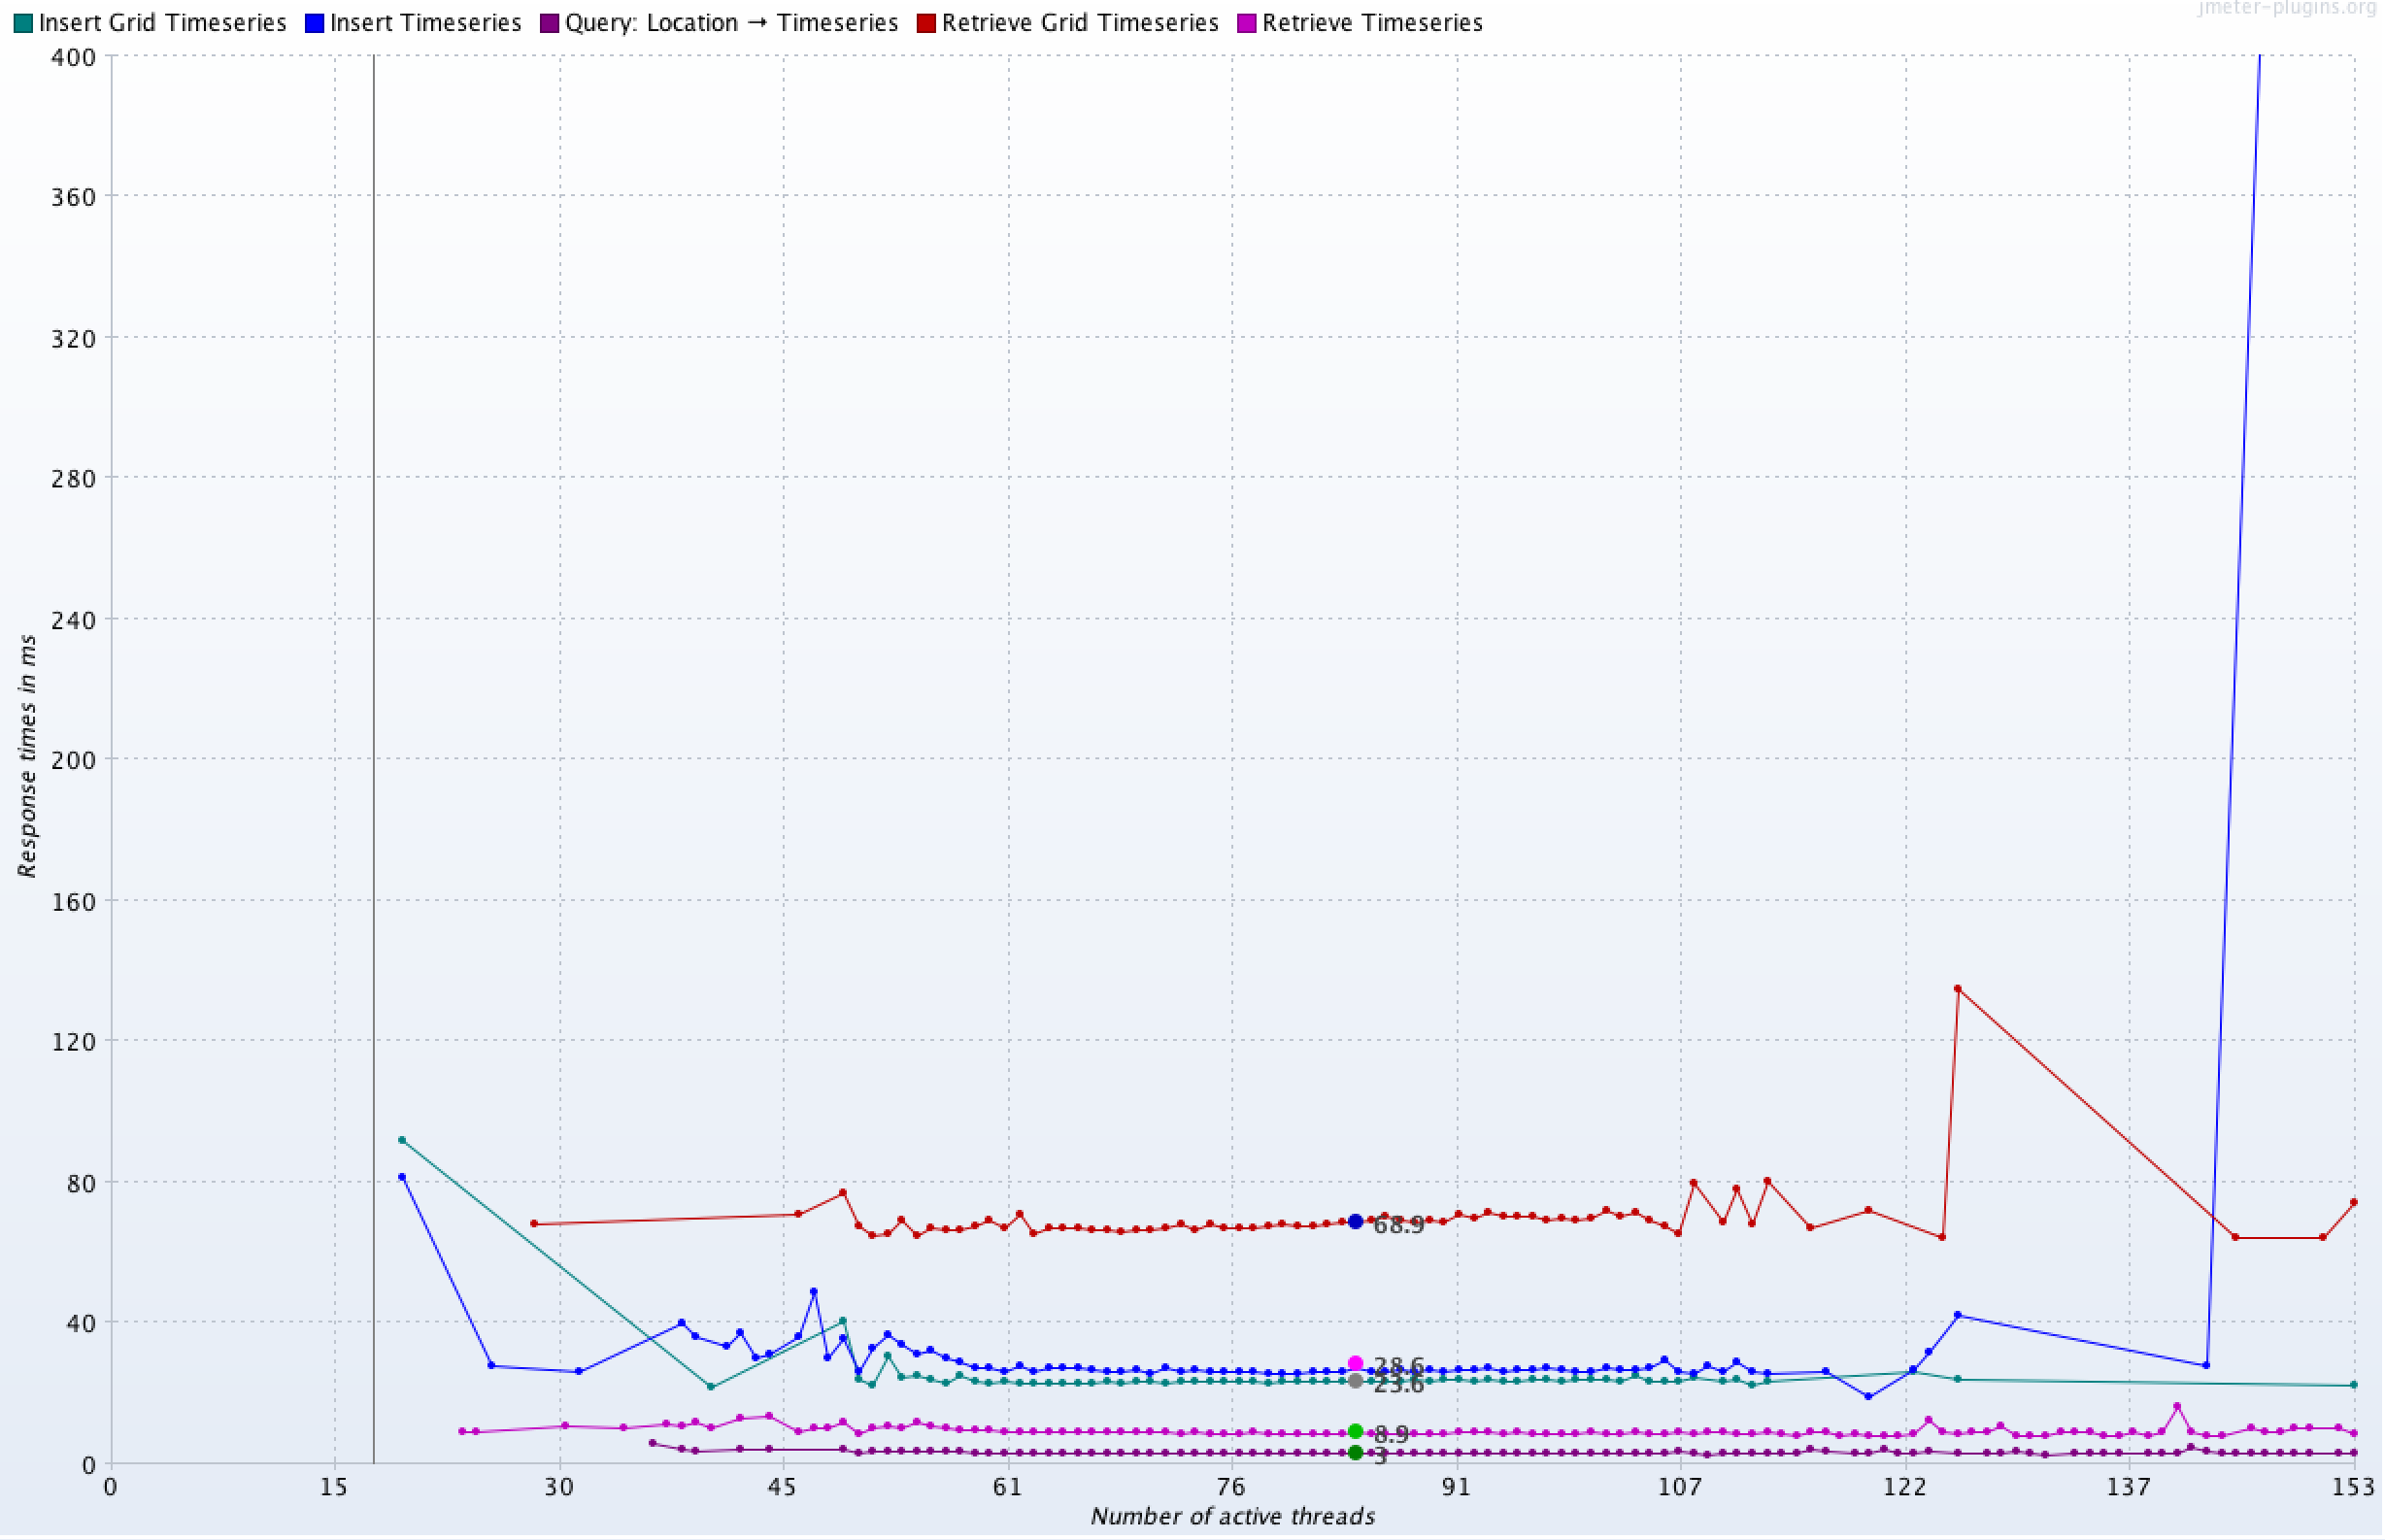
\includegraphics[width=1.0\textwidth]{results/obs/all/obs_all_60m_response_times_vs_threads.png}
    \caption{Response time vs threads while load testing with hourly data.}
    \label{fi:test_obs_all_60m_response_vs_threads}
\end{figure}
\cref{fi:test_obs_all_60m_response_vs_threads} shows the response time against the number of active threads for 60-minute data requests. As the graph shows, the response time kept the same while increasing the number of active threads against each test case. The above graph shows the scalability of the \acrshort{wdias} since the system is able to process more requests without a significant change in the latency. When the number of active threads increased more than 122, \cref{fi:test_obs_all_60m_response_vs_threads} shows uncertainty in the inserting and retrieving scalar and vector data. The performance degrades because those data handles on-demand and depends on the timeseries database performance. 
However, when the request sizes are smaller, \acrshort{wdias} was able to perform insert and retrieval of grid data with the same latency.

\begin{figure}[htp]
    \centering
    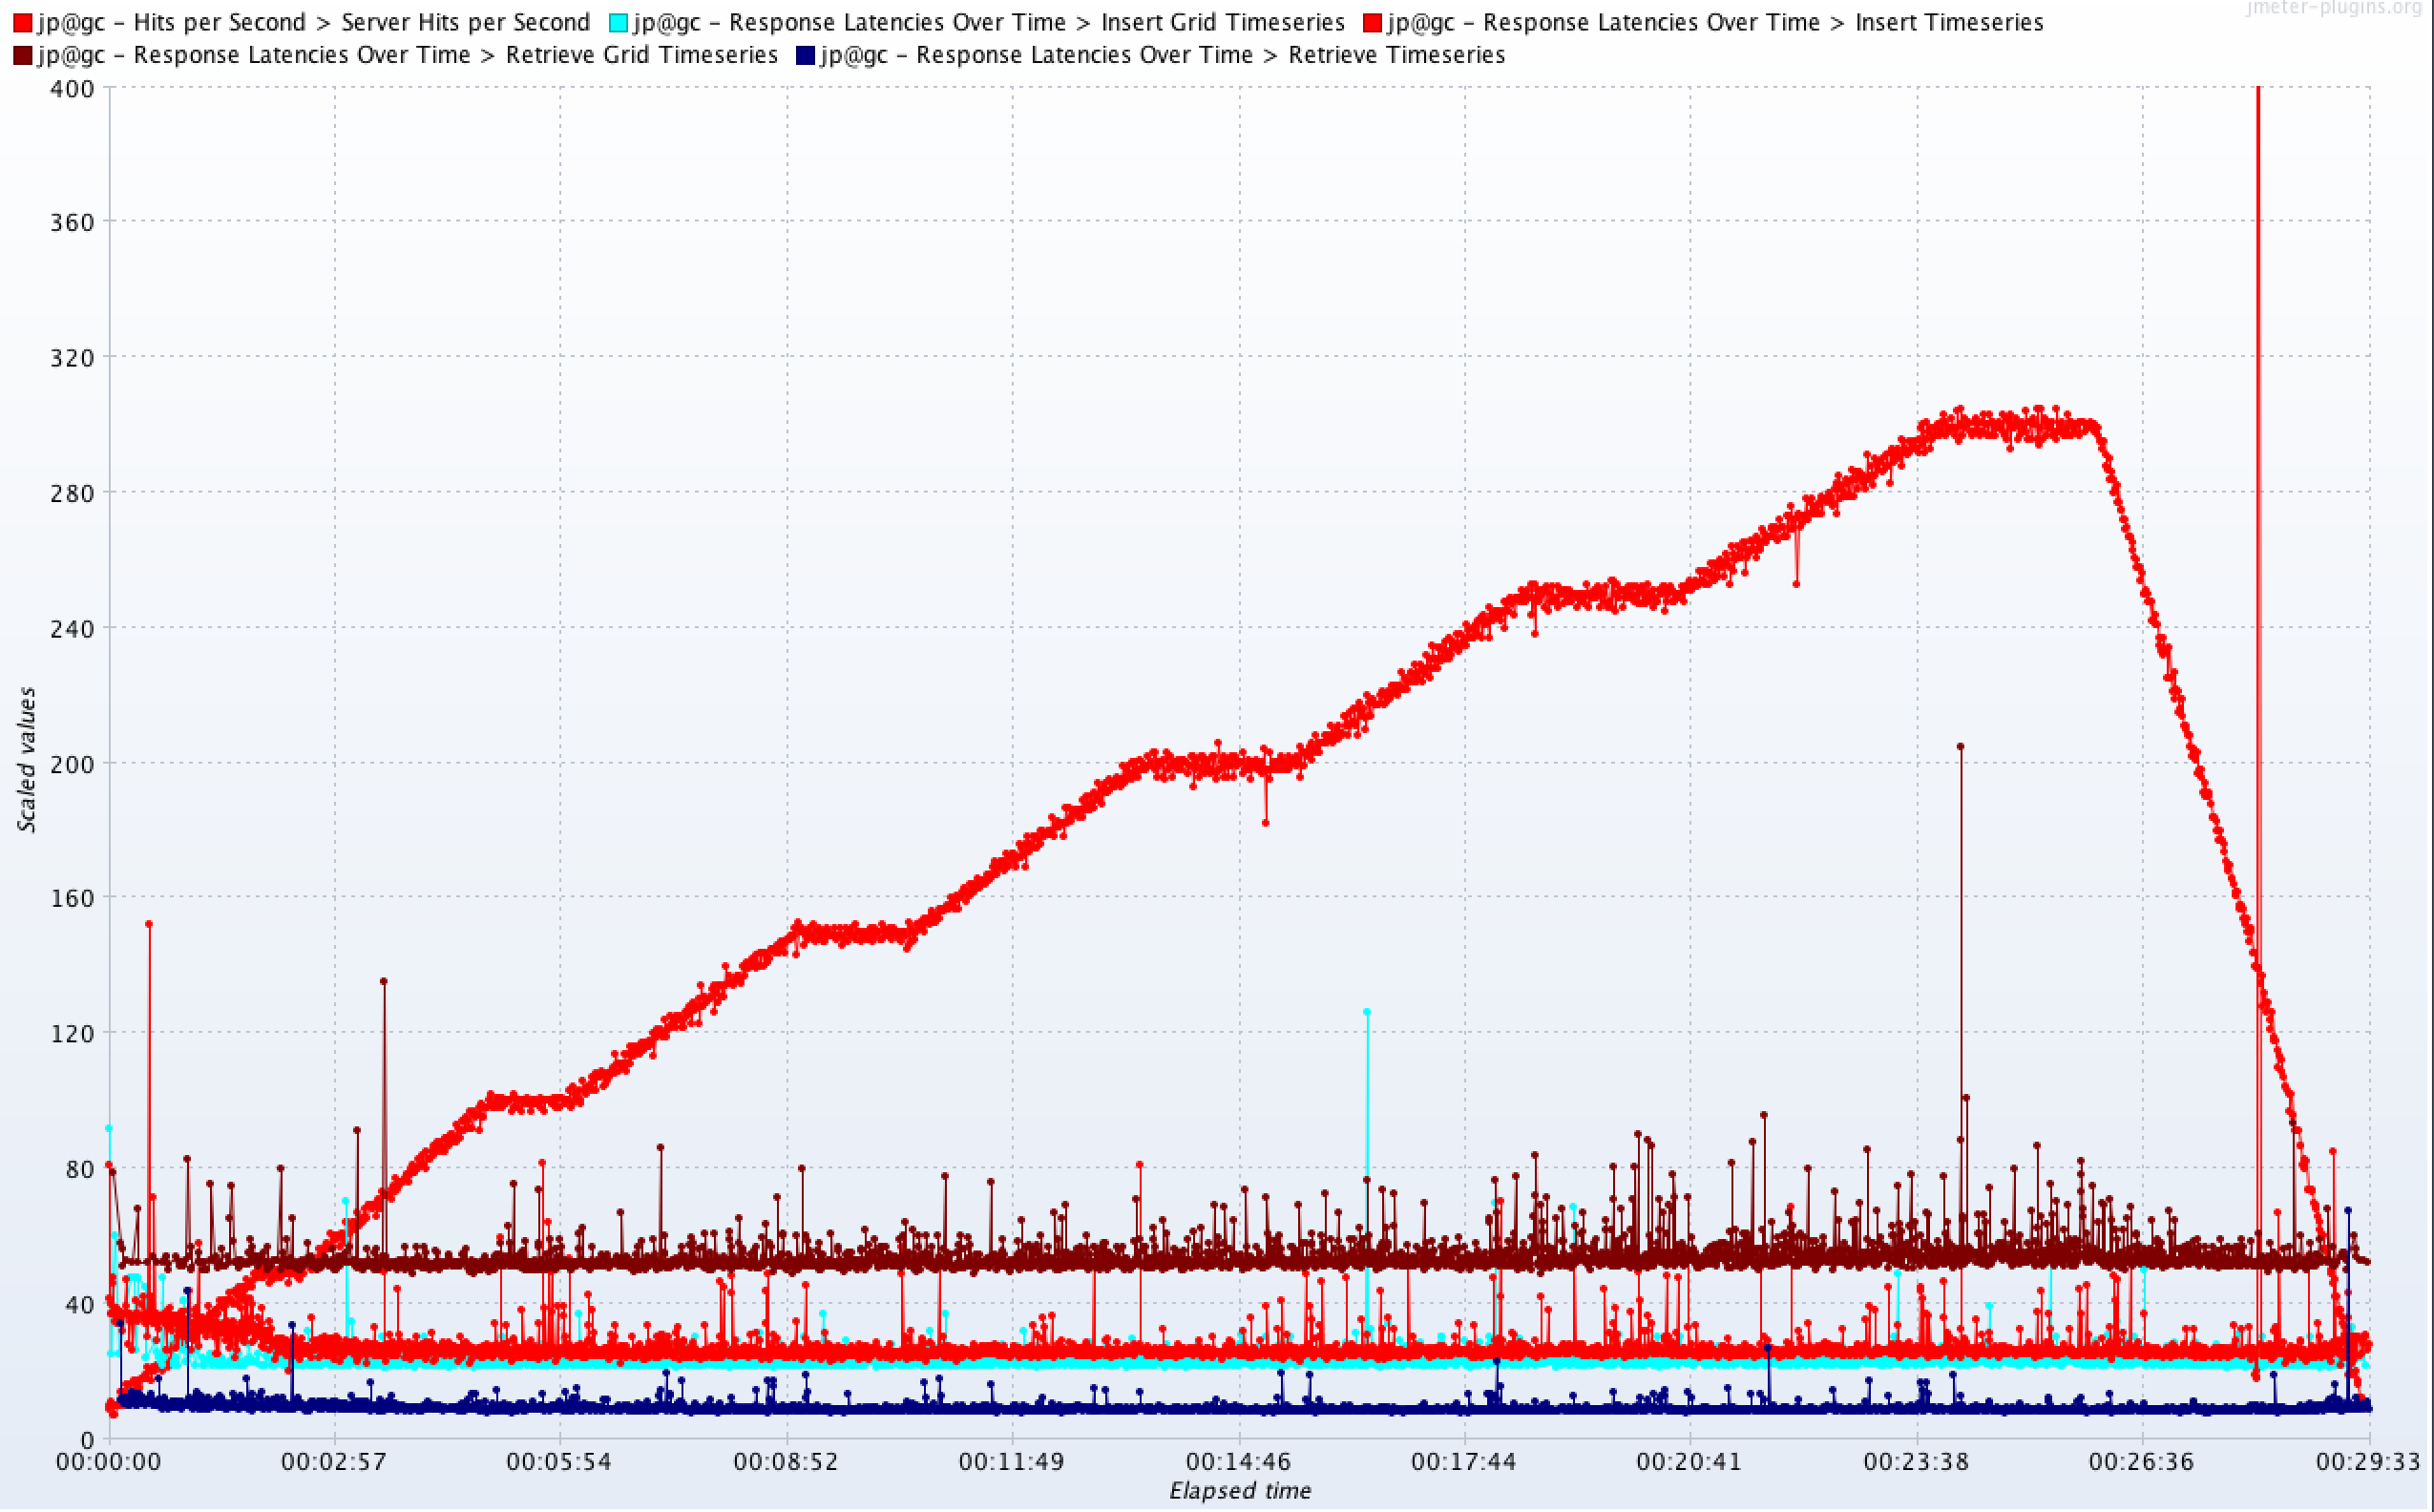
\includegraphics[width=1.0\textwidth]{results/obs/all/obs_all_60m_res_latencies_against_hits.png}
    \caption{Latency against server hits while load testing with hourly data.}
    \label{fi:test_obs_all_60m_latency}
\end{figure}

\cref{fi:test_obs_all_60m_latency} graph provides a better overview of the variation of latency over the elapsed time of the test plan against the number of server hits per second. This graph further proves that the system was able to handle the increasing workload without any significant change in the delay. The stepped red colour graph for server hits per second shows the number of requests that was sent by the load test with time. Other horizontal lines with spikes show the latency for each of test case, such as insertion and retrieval of scalar, vector, and grid data with time.


%%%%%%%%%%%%%%%%%%%%%%%%%%%%%%%%%%%%%%%%%%%%%%%%%%%%%%%%%%%%%%%%%%%%%%%%%%%%%%%%
\subsection{Load Testing with 30-minute Resolution Data}
\label{subse:obs_test_plan_all_30min}

Next, we performed the test plan with 30-minute resolution data, which means 48 data points per each request for the scalar and vector data types, and 48 ASCII grid files with 2.4 MB of size per each insertion request for the grid data type. Also, the test plan performed round up to \num{311e3} number of sample requests, which is almost similar to the number of samples processed with hourly resolution data. That means \acrshort{wdias}-based system was able to process same number of request while increasing the request size with providing higher throughput.

\begin{table}[ht]
\caption{Throughput and latency of load test with 30-minute data}
\footnotesize
\begin{tabulary}{\linewidth}{|L|R|R|R|R|R|R|R|R|}
\hline
\textbf{Label} & \textbf{Samples} & \textbf{Avg} & \textbf{Min} & \textbf{Max} & \textbf{90\% Line} & \textbf{Std.Dev.} & \textbf{Error} & \textbf{RPS} \\ \hline
Insert Timeseries & 71759 & 29 & 14 & 1699 & 32 & 50.97 & 0.00\% & 40.5 \\ \hline
Retrieve Timeseries & 71730 & 9 & 7 & 1033 & 10 & 6.04 & 0.00\% & 40.6 \\ \hline
Insert Grid & 7972 & 44 & 40 & 162 & 49 & 8.17 & 0.08\% & 4.5 \\ \hline
Retrieve Grid & 7971 & 81 & 67 & 284 & 93 & 15.15 & 0.00\% & 4.5 \\ \hline
Query: Location & 71734 & 3 & 2 & 110 & 3 & 1.90 & 0.00\% & 40.5 \\ \hline
TOTAL & 310878 & 129 & 0 & 1699 & 503 & 207.10 & 0.00\% & 175.3 \\ \hline
\end{tabulary}
\label{tab:obs_all_30_min_summary}
\end{table}

\cref{tab:obs_all_30_min_summary} shows the response latency summary details and \acrshort{rps} with 30-minute resolution data. The results are almost similar to the observations in \cref{subse:obs_test_plan_all_60min}. Even though we doubled the request size, \acrshort{wdias} was able to keep the performance almost the same instead of increasing the latency twice.
Insertion and retrieval of scalar and vector data increased by 1 millisecond on average. However, the grid data insert latency increased from 23 milliseconds to 40 milliseconds. Such doubling of latency is expected, as the grid data size was increased from 1.2 MB to 2.4 MB, and it is taking time to stream the data into \acrshort{wdias}-based system. Retrieval of grid data also increased by 22 milliseconds, because during the test cases, we try to retrieve the inserted grid data in a different format, but the export data size also gets increased due to the increase of the insert grid data size.

\begin{figure}[htp]
    \centering
    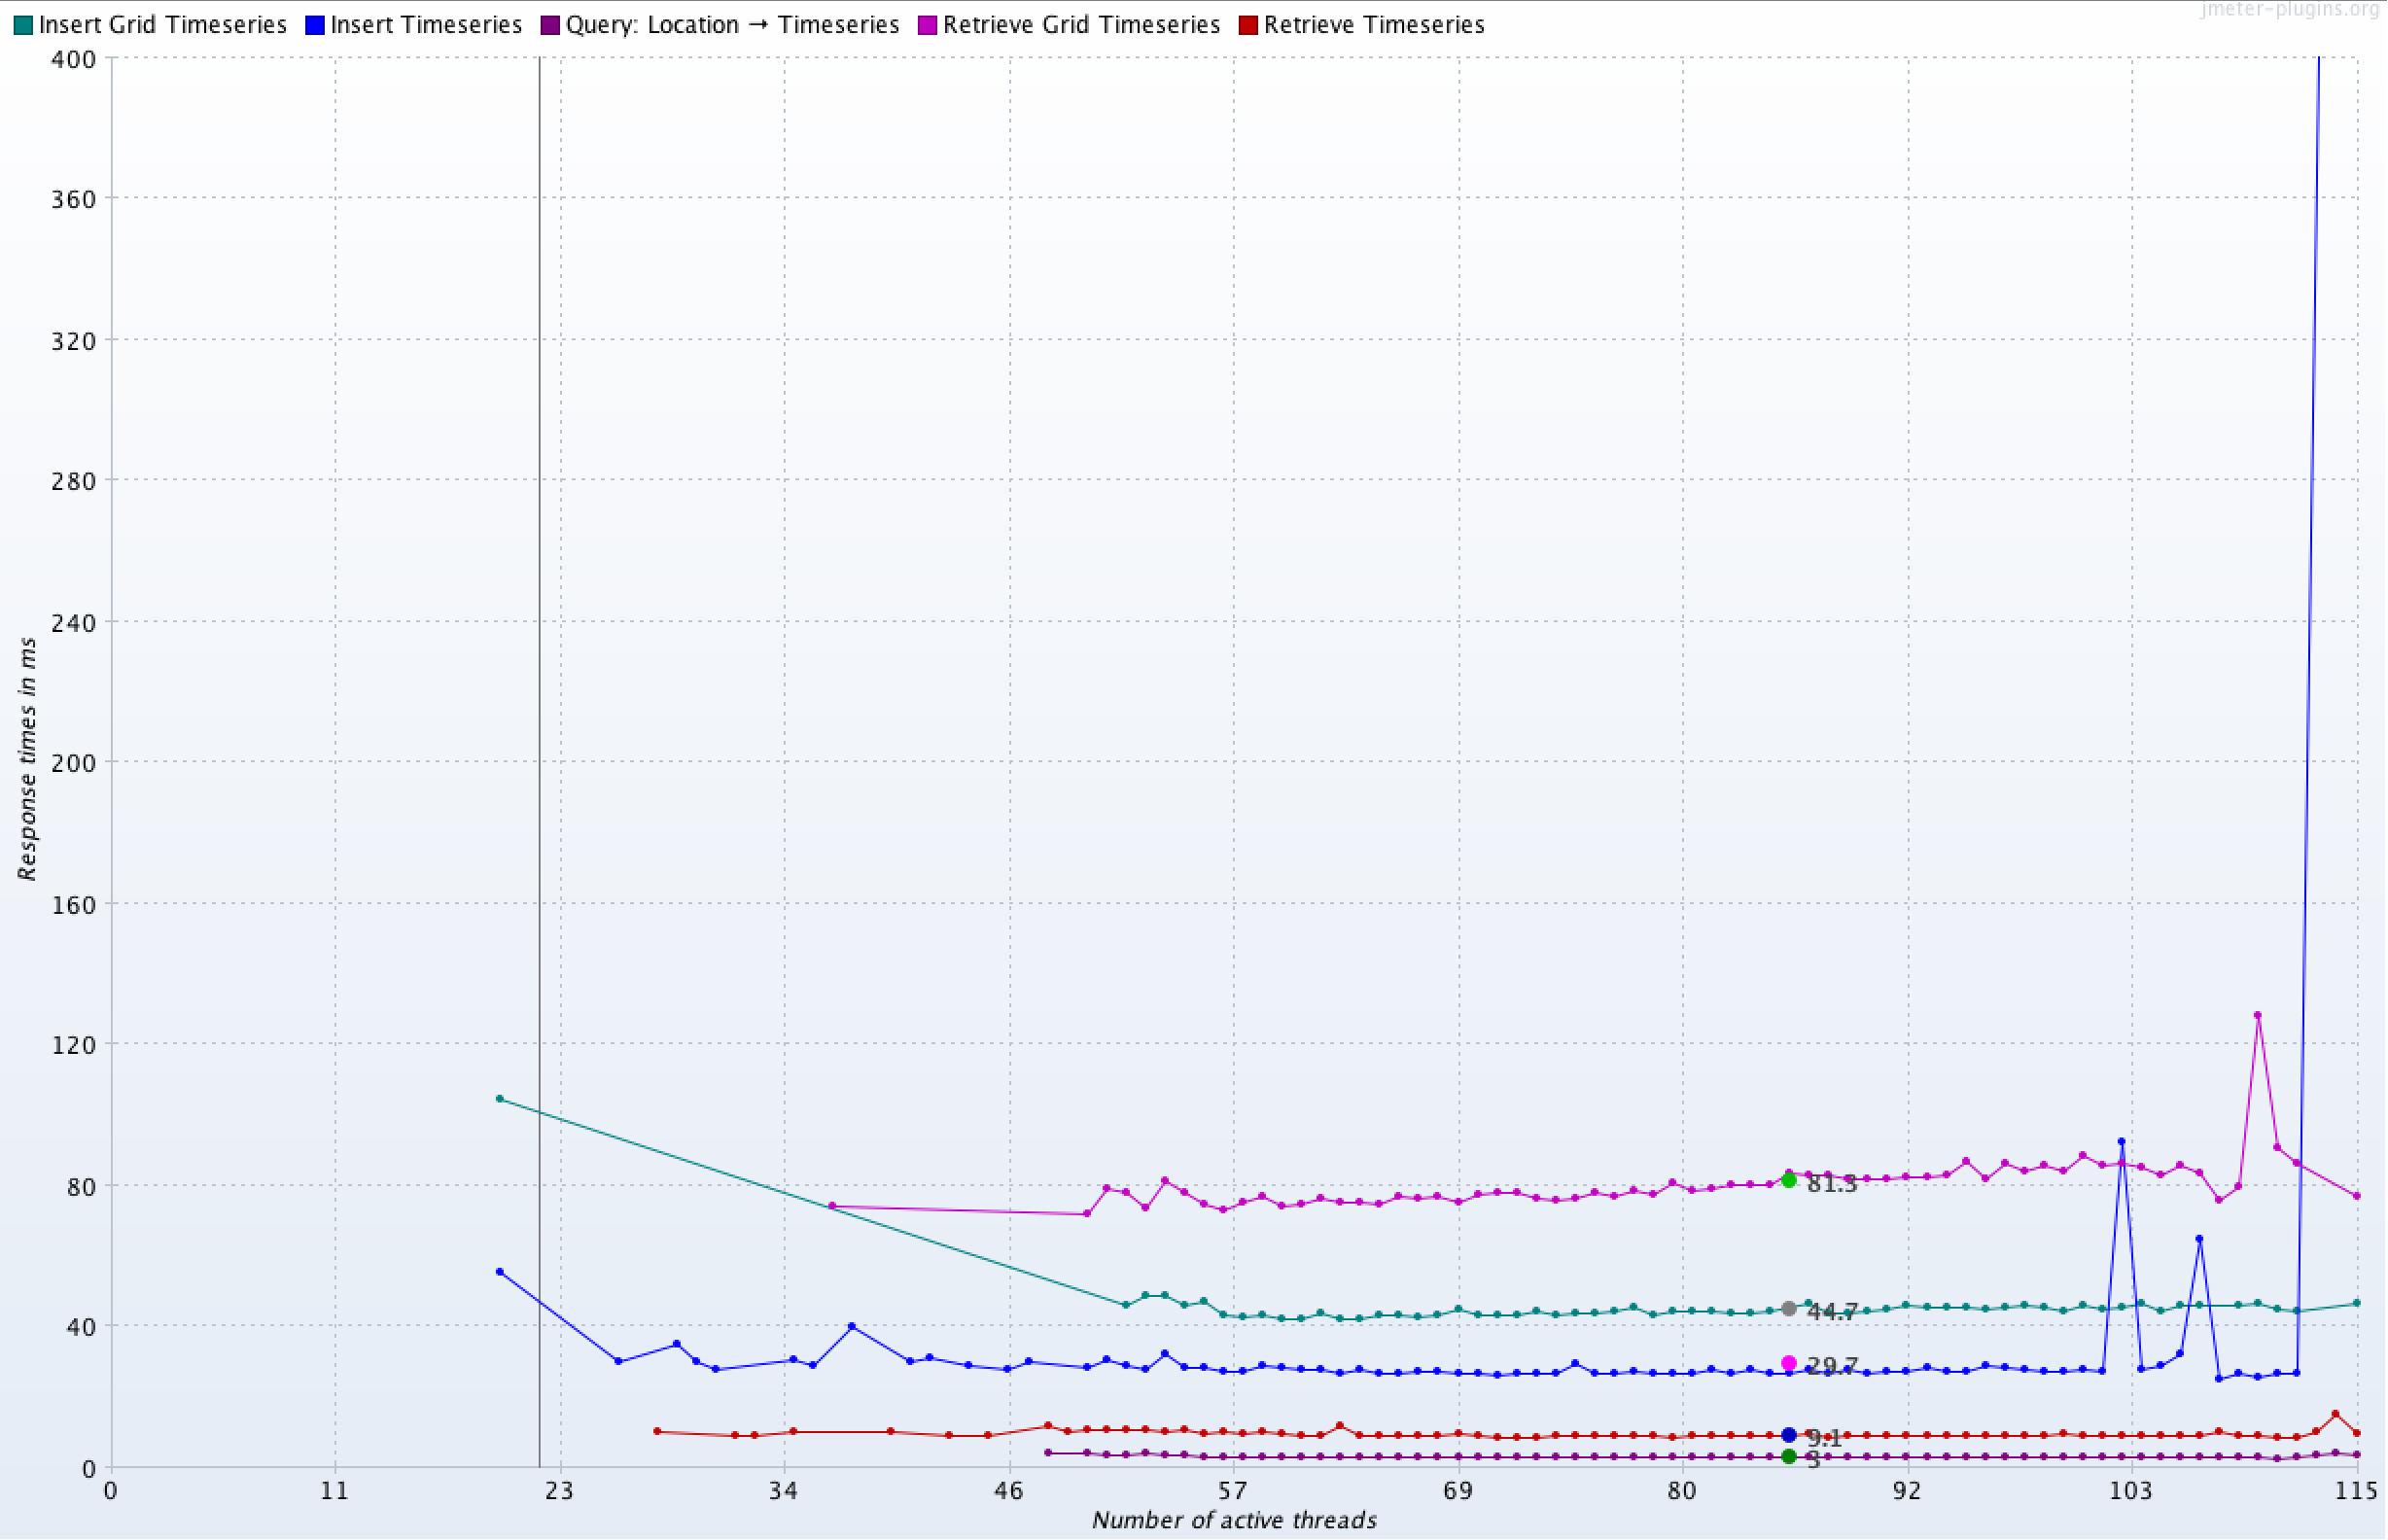
\includegraphics[width=1.0\textwidth]{results/obs/all/obs_all_30m_response_times_vs_threads.png}
    \caption{Response time vs threads while load testing with 30-minute of data.}
    \label{fi:test_obs_all_30m_response_vs_threads}
\end{figure}

\cref{fi:test_obs_all_30m_response_vs_threads} shows the latency against the number of active threads for the test plan with 30-minute resolution data. As the graph shows, the response time kept almost constant while increasing the number of active threads. Thus, we can say that \acrshort{wdias} is a scalable system since it was able to increase the throughput without a significant change in the latency. When the number of active threads increased, \cref{fi:test_obs_all_30m_response_vs_threads} shows uncertainty in the insertion and retrieval of scalar and vector data. Some of the facts cause this is, those operations are handled on-demand. At the same time, the system is writing timeseries while reading from the timeseries database. The InfluxDB can fine-tune for writes or read based on the requirements, but we used it with default configurations. Also, the InfluxDB commercial version support horizontal database scaling with sharding, and we are using the basic open source support in this test setup.

\begin{figure}[htp]
    \centering
    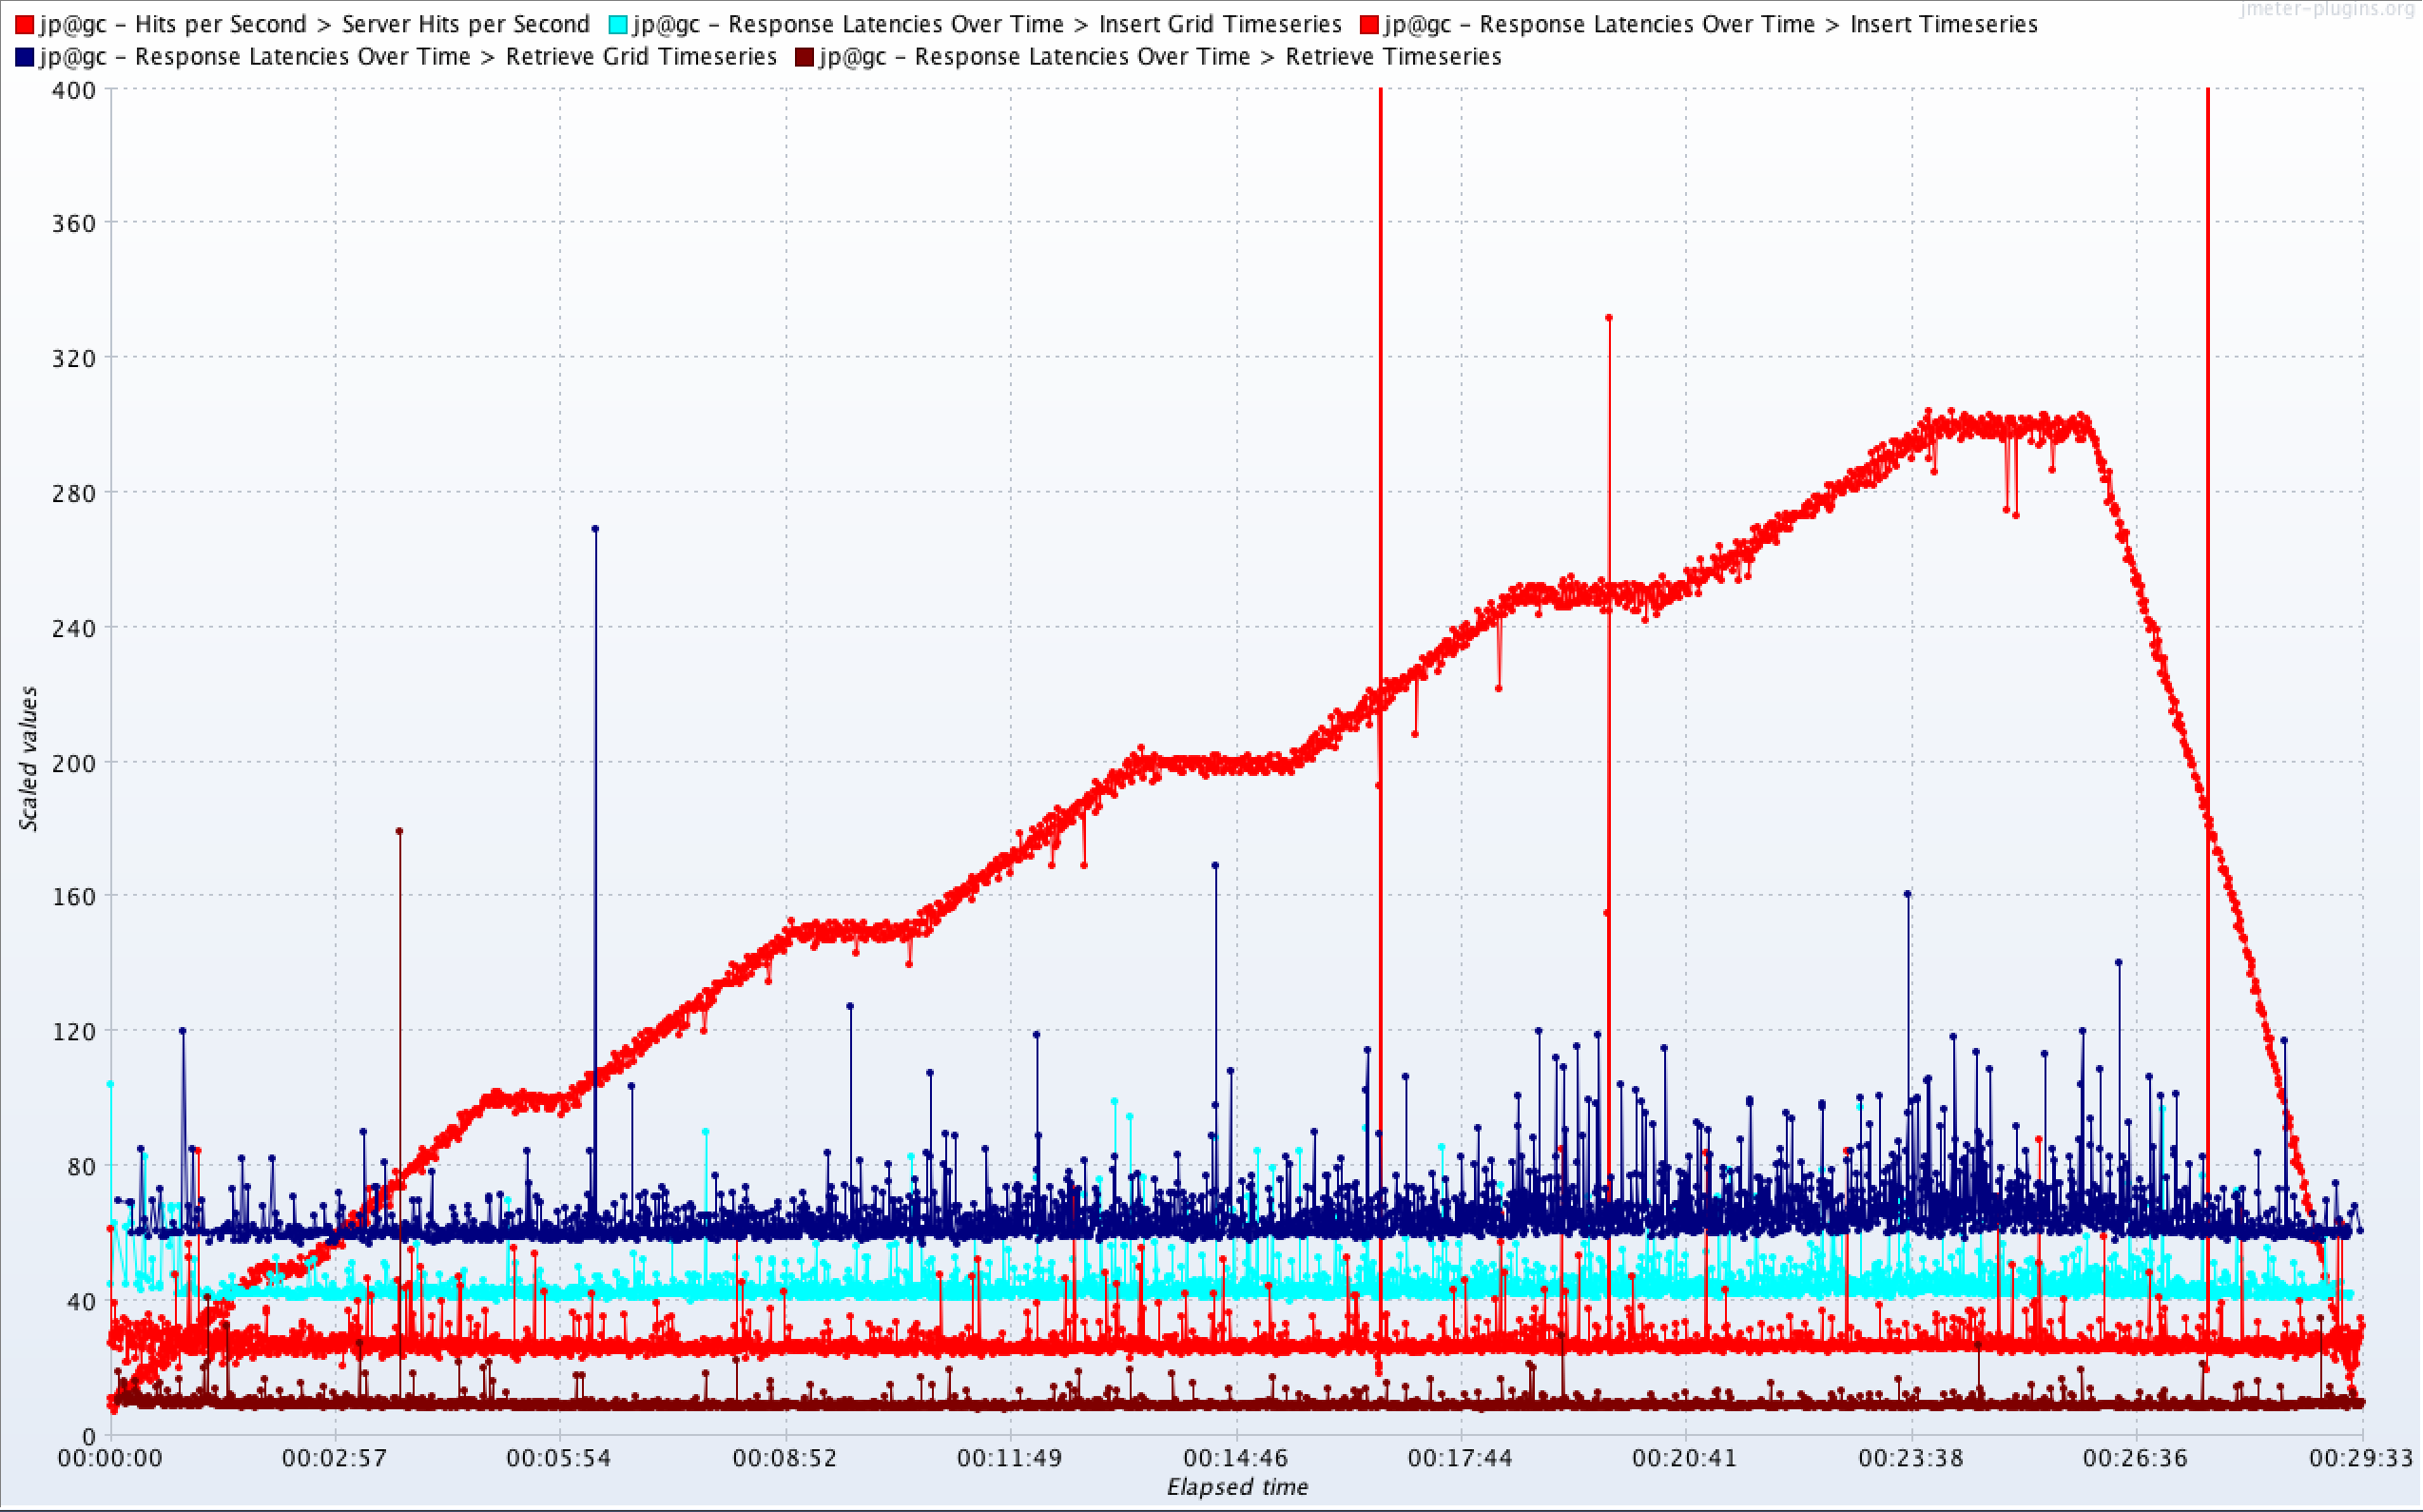
\includegraphics[width=1.0\textwidth]{results/obs/all/obs_all_30m_res_latencies_against_hits.png}
    \caption{Latency against server hits while load testing with 30 minute of data.}
    \label{fi:test_obs_all_30m_latency}
\end{figure}
\cref{fi:test_obs_all_30m_latency} graph provides a better overview of the variation of latency over the elapsed time of the test plan against the \acrshort{rps}. By referring to the graph, we can see that over the elapsed time the latency does not change very significantly. However, during the peak load, it shows a minor spikes in latency of the insertion and retrieval of grid timeseries. When compared to \cref{fi:test_obs_all_60m_latency}, the latency of insertion grid timeseries data almost doubled. The grid timeseries data was handled asynchronously after successfully steamed the data into the \acrshort{wdias} system, thus the latency for storing the data increased by a factor of two since the request data size also increased twice.


%%%%%%%%%%%%%%%%%%%%%%%%%%%%%%%%%%%%%%%%%%%%%%%%%%%%%%%%%%%%%%%%%%%%%%%%%%%%%%%%
\subsection{Load Testing with 15-minute Resolution Data}
\label{subse:obs_test_plan_all_15min}

During this section, we performed the test plan with 15-minute resolution data, which means 96 data points per each request for the scalar and vector data types, and 96 ASCII grid files per each insertion request with the size of 4.9 MB for the grid data type. The size of each request is four times larger than the 60-minute resolution data. Here also, the test plan performed approximately \num{311e3} of sample requests, which are almost similar to sample requests made during 60-minute and 30-minute resolution data. This means \acrshort{wdias}-based system was able to increase the throughput while increasing load with the request size, and processed the same amount of requests within the elapsed time.

\begin{table}[ht]
\caption{Throughput and latency of load test with 15-minute data}
\footnotesize
\begin{tabulary}{\linewidth}{|L|R|R|R|R|R|R|R|R|}
\hline
\textbf{Label} & \textbf{Samples} & \textbf{Avg} & \textbf{Min} & \textbf{Max} & \textbf{90\% Line} & \textbf{Std.Dev.} & \textbf{Error} & \textbf{RPS} \\ \hline
Insert Timeseries & 71775 & 30 & 12 & 1719 & 41 & 51.71 & 0.00\% & 40.5 \\ \hline
Retrieve Timeseries & 71736 & 23 & 8 & 1623 & 32 & 50.18 & 0.00\% & 40.6 \\ \hline
Insert Grid & 7975 & 91 & 77 & 279 & 112 & 19.58 & 1.42\% & 4.5 \\ \hline
Retrieve Grid & 7972 & 118 & 80 & 876 & 165 & 56.15 & 0.00\% & 4.5 \\ \hline
Query: Location & 71749 & 3 & 2 & 130 & 4 & 2.32 & 0.00\% & 40.5 \\ \hline
\textbf{TOTAL} & 310934 & 134 & 0 & 1719 & 503 & 206.40 & 0.04\% & 175.4 \\ \hline
\end{tabulary}
\label{tab:obs_all_15_min_summary}
\end{table}

\cref{tab:obs_all_15_min_summary} shows the response latency summary details and \acrshort{rps} of the test plan with 15-minute resolution data. When compared to the observations from the performance test with 30-minute data, the request latency also increased for all sample requests. The scalar and vector data insertion increased by 1 milliseconds, and retrieval of those data increased significantly by doubling the latency. Also, the standard deviation of retrieval timeseries data increased by a considerable amount for all the data type's sample requests. One of the reasons for increasing the retrieval data delay was while performing heavy database writes on the InfluxDB database instance has effects on the database reads. The grid data insert and retrieve latency also doubled approximately because the stream data size increase by a factor of two compared to 30-minute data. Noticeably, the error rate of inserting grid data increased up to 1.42\%. Even though we increased the request data size by four times higher, the system was able to handle all requests without significant performance issues. Also, the system was able to process same number of request as with 60-minute and 30-minute resolution data while increasing the throughput of the system with the request size.

\begin{figure}[htp]
    \centering
    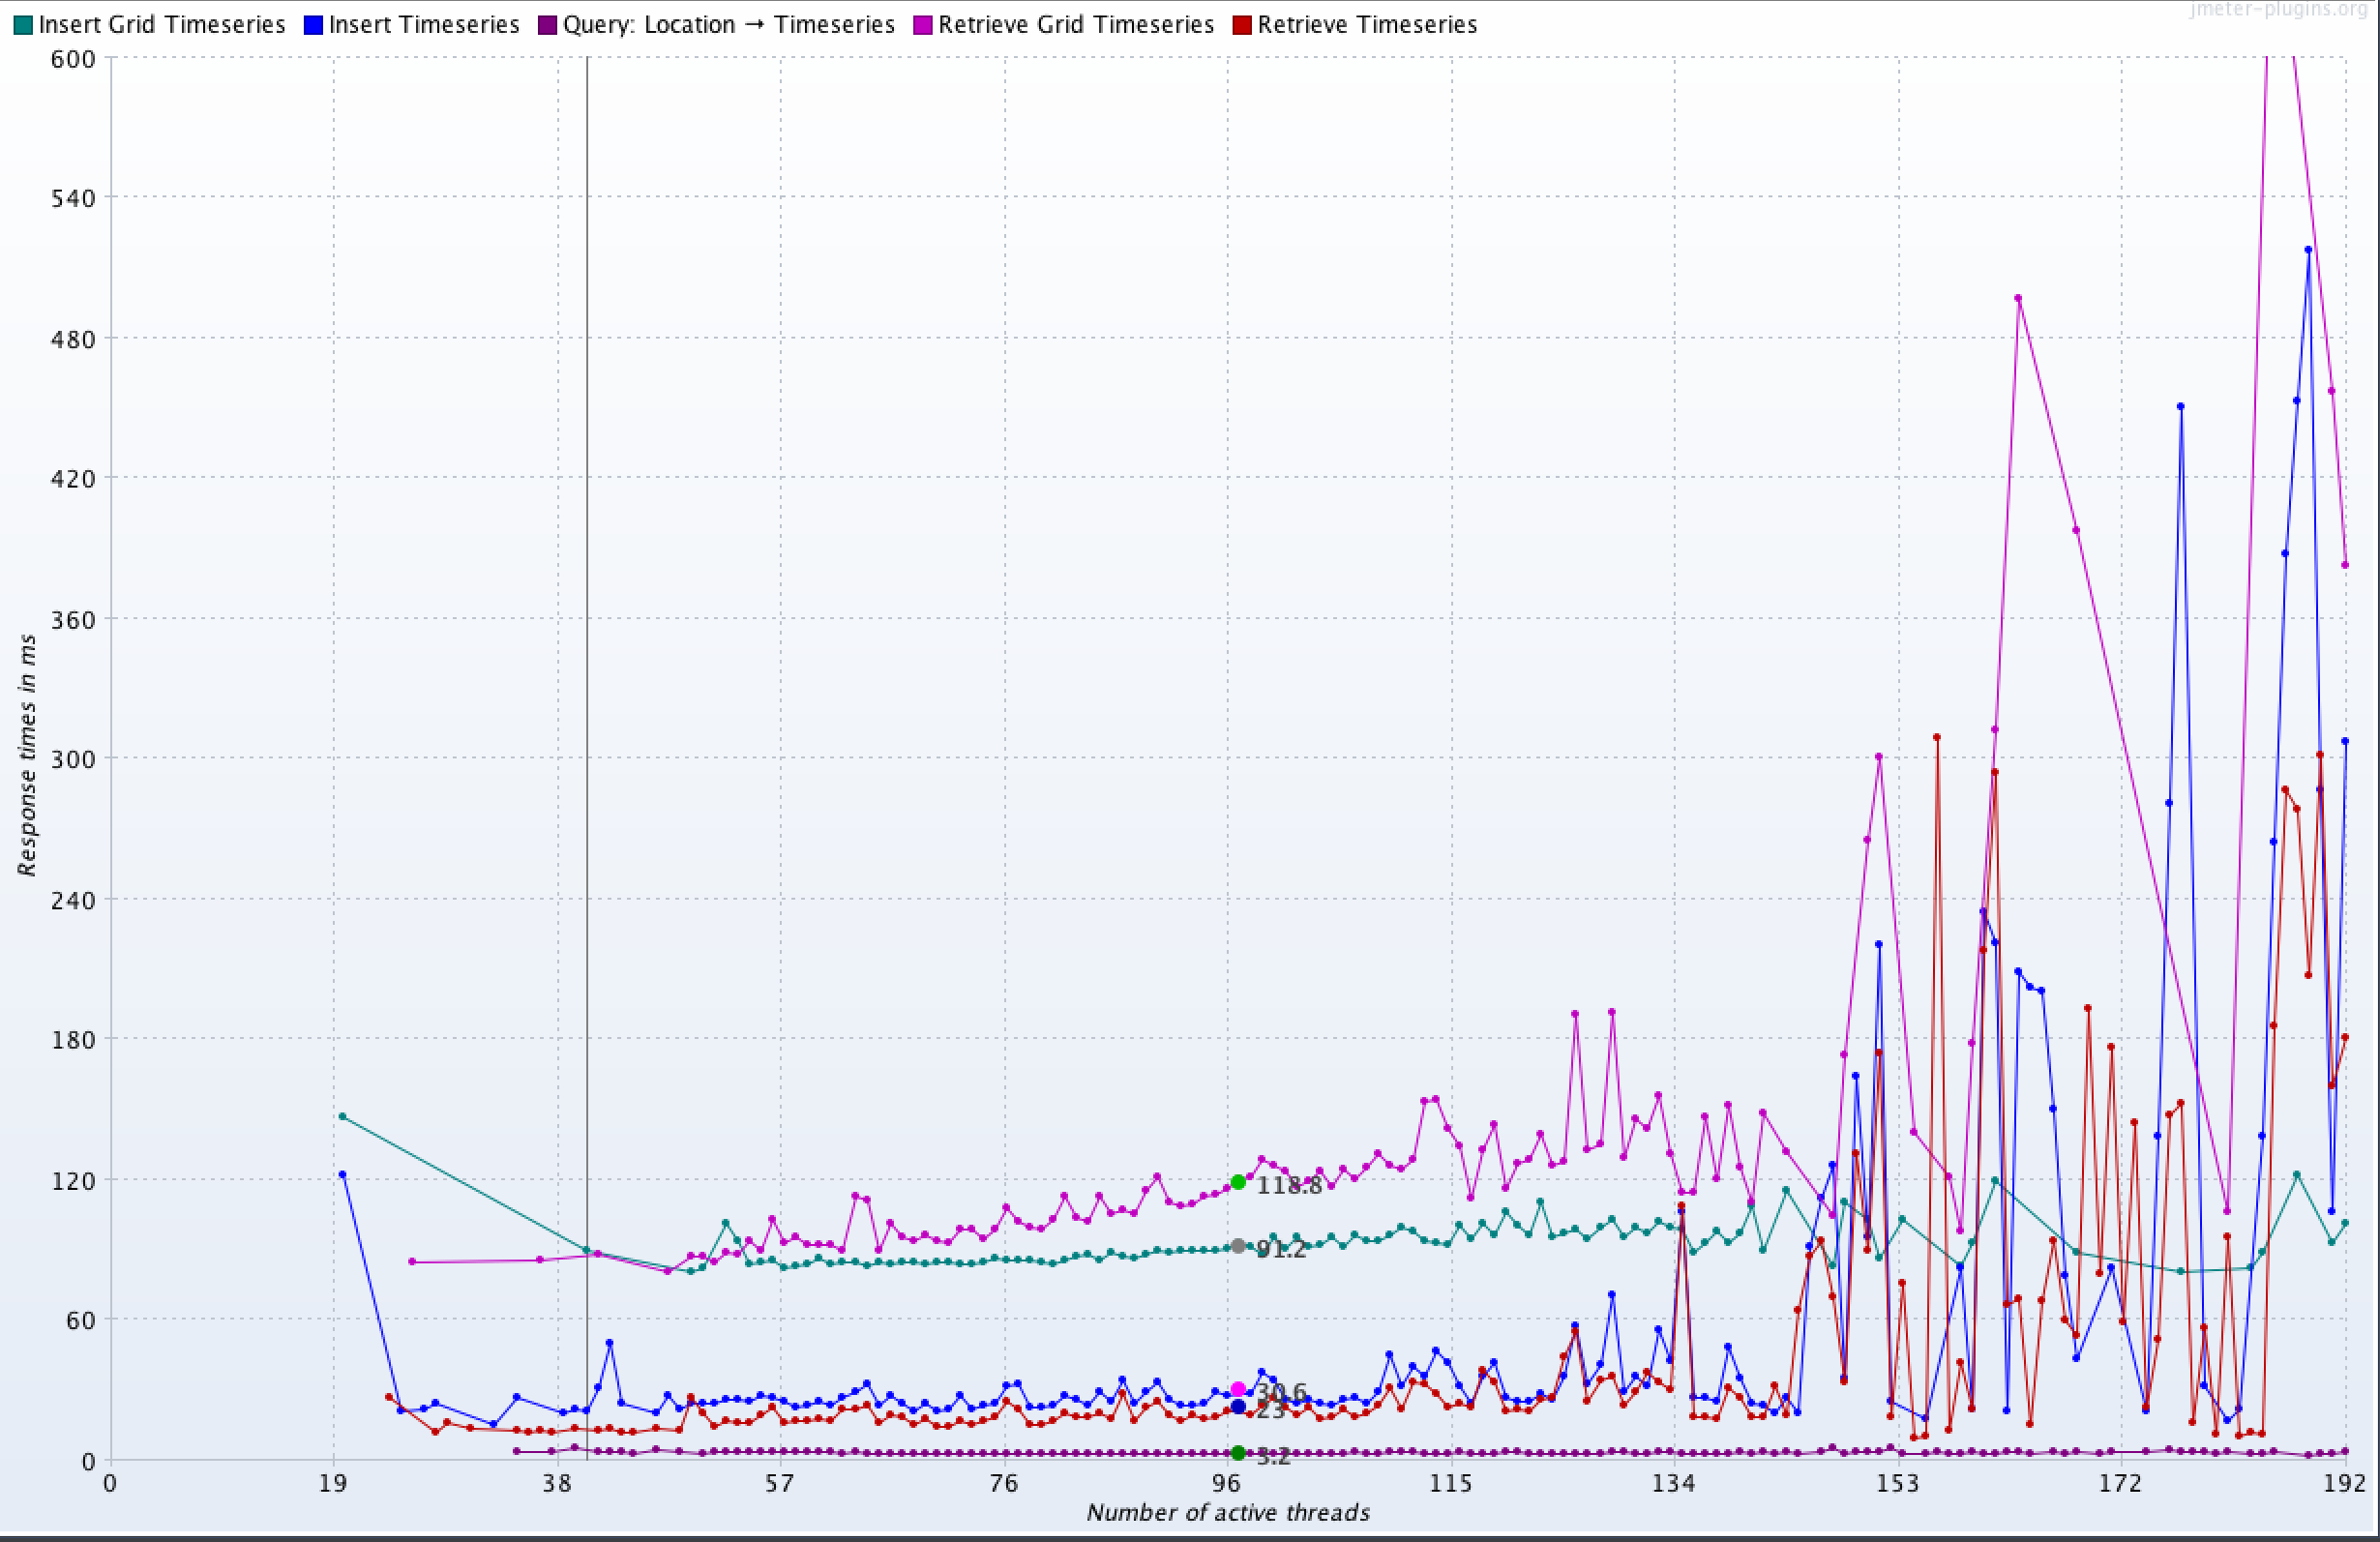
\includegraphics[width=1.0\textwidth]{results/obs/all/obs_all_15m_response_times_vs_threads.png}
    \caption{Response time vs active threads while load testing with 15-minute of data.}
    \label{fi:test_obs_all_15m_response_vs_threads}
\end{figure}

\cref{fi:test_obs_all_15m_response_vs_threads} shows the latency against the number of active threads for the test plan with 15-minute resolution data. As per the graph, the system was able to keep the response latency constant while increasing the number of active threads. However, when the number of active threads became higher, there was a disturbance with the response delay during the insertion and retrieval of scalar and vector timeseries data. As mentioned above, this may happened due to the system reaching its maximum capacity as per the allocated resources, or caused by heavy database read and writes on the InfluxDB free database version. The latency of insert and retrieval of grid timeseries data increased twice when compared to 30-minute resolution data. With a larger request size, we can notice the latency also increased by a smaller factor when we increased the number of active threads. When compared to the load testing with 60-minute and 30-minute data, we can see 192 active threads used by the JMeter to maintain the \acrshort{rps}. When we increase the request size, the latency also increases. Then the active threads have to wait for the response from the system rather than doing any other work. To maintain the server hits, the JMeter has to spawn more active threads.

\begin{figure}[htp]
    \centering
    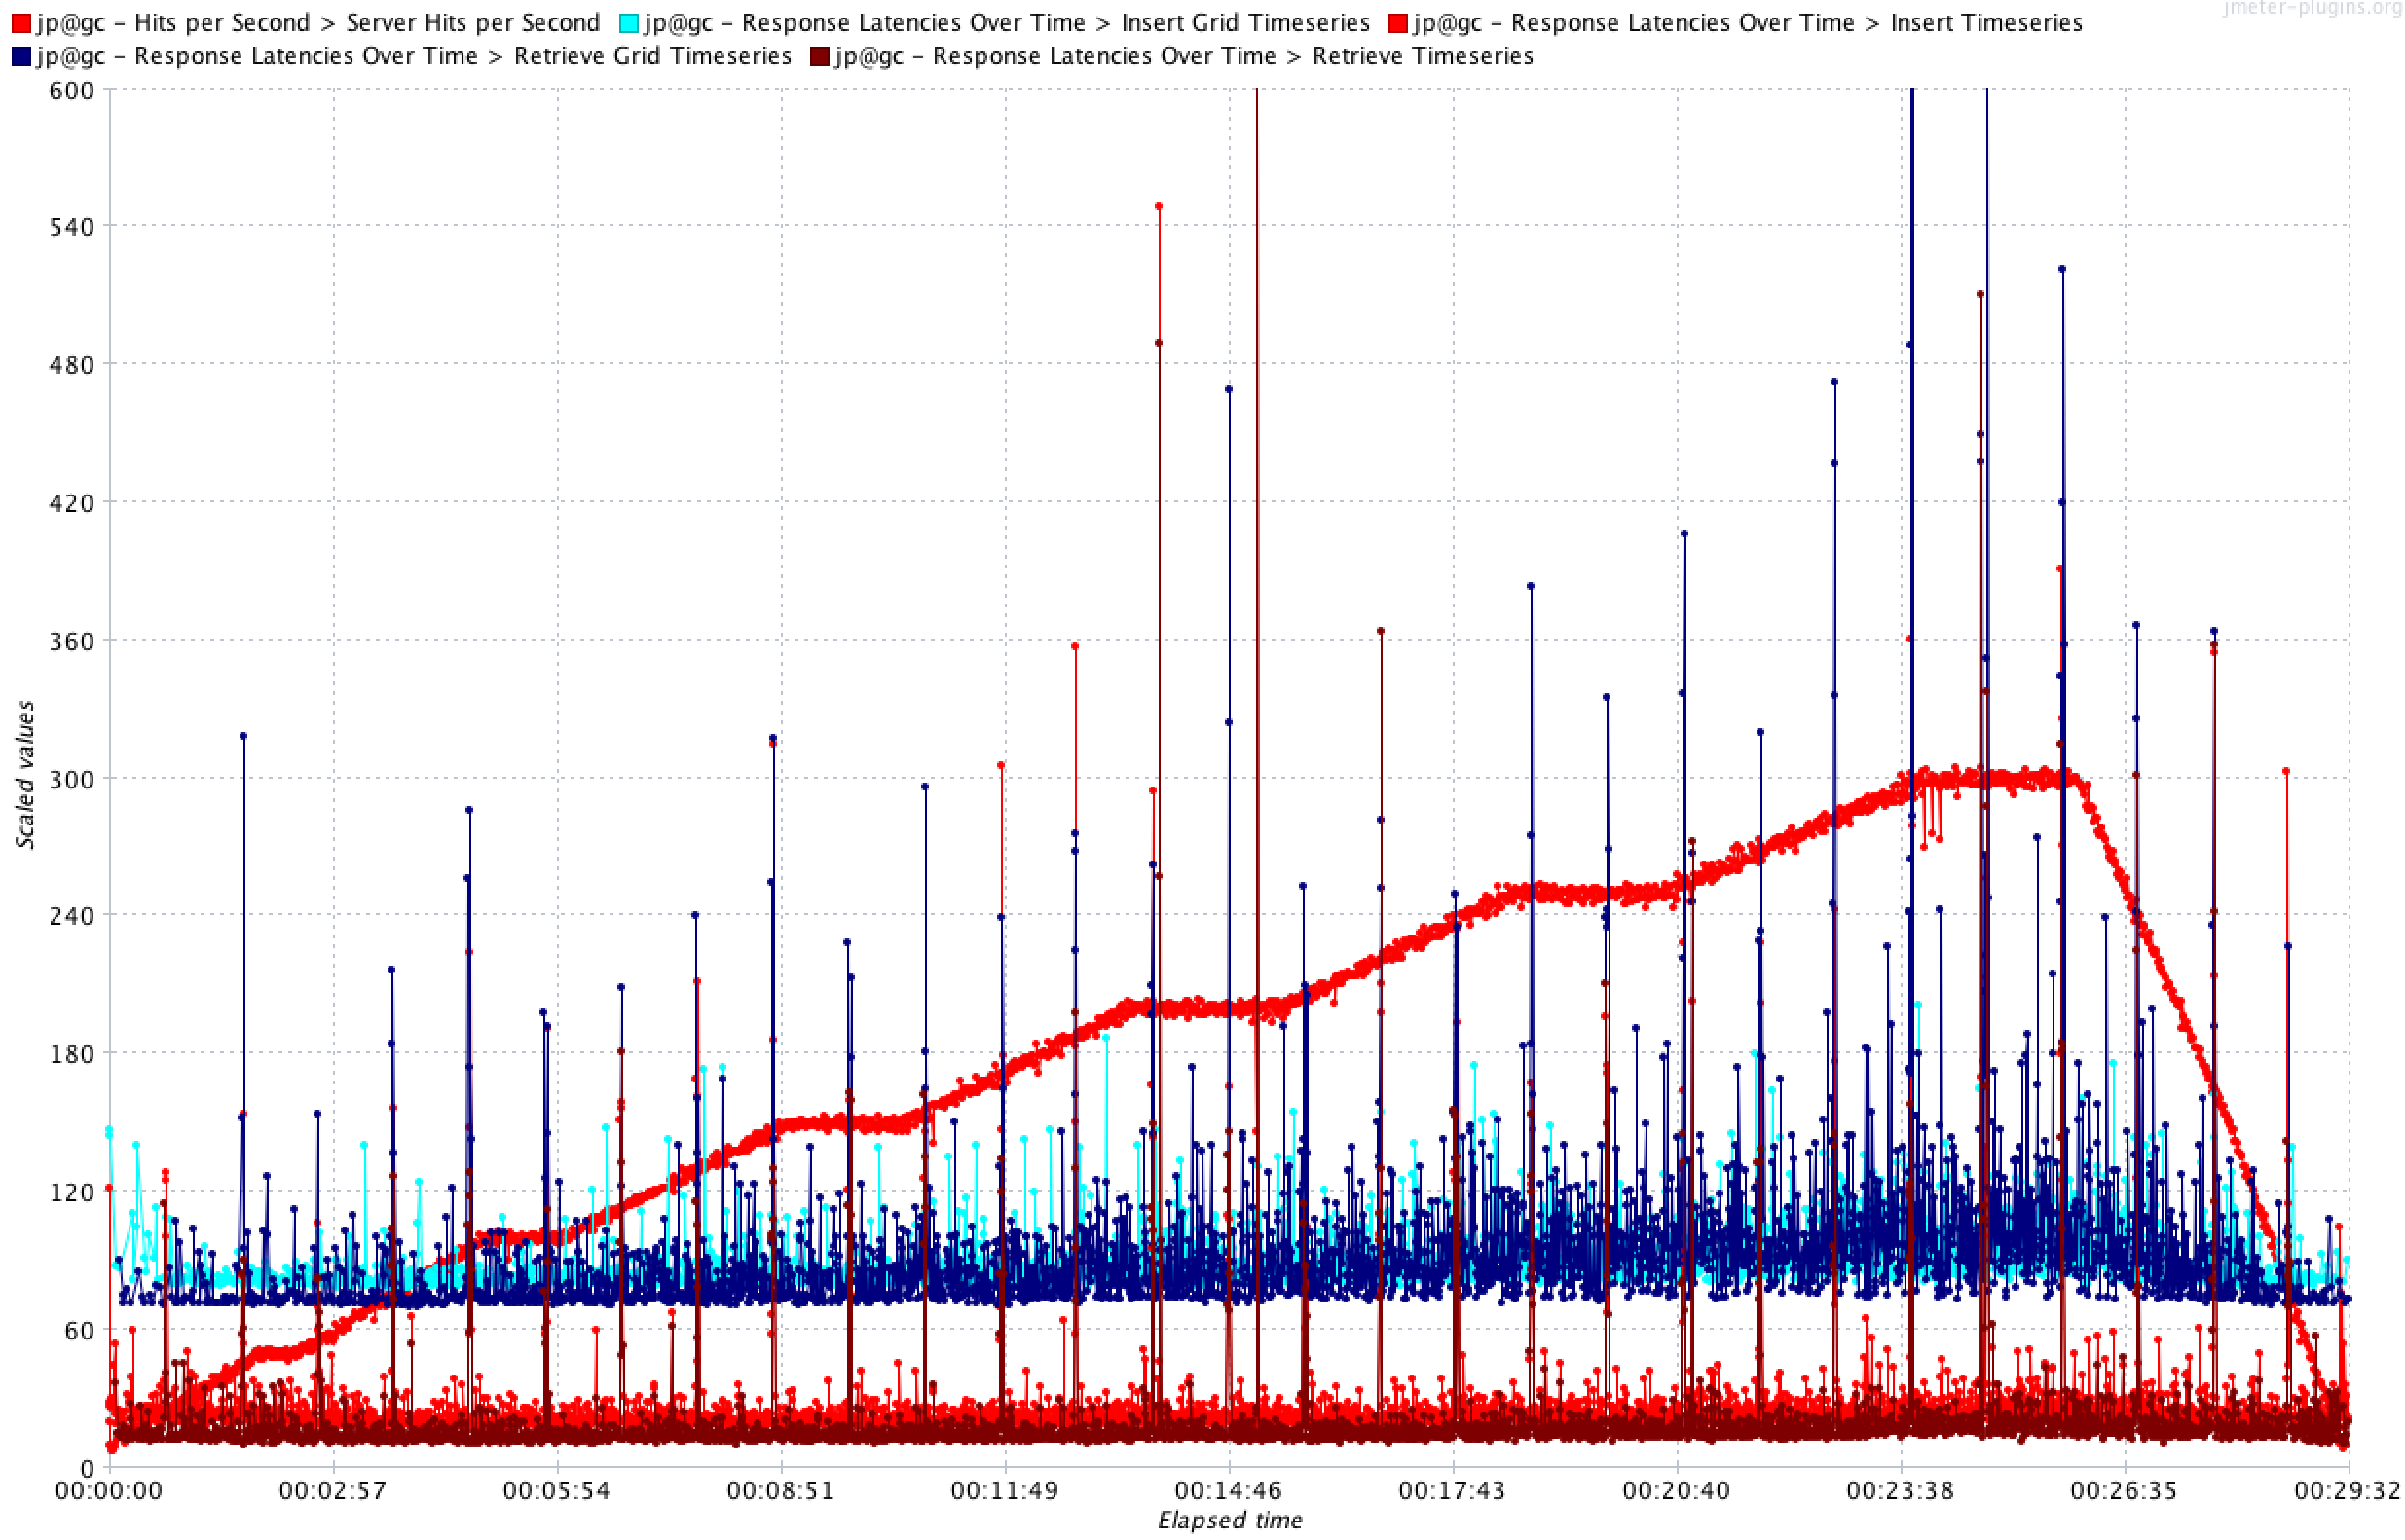
\includegraphics[width=1.0\textwidth]{results/obs/all/obs_all_15m_res_latencies_against_hits.png}
    \caption{Latency against server hits while load testing with 15-minute of data.}
    \label{fi:test_obs_all_15m_latency}
\end{figure}

\cref{fi:test_obs_all_15m_latency} graph provides an overview of the variation of latency over the elapsed time of the test plan against the number of server hits per second for 15-minute resolution data. As per the graph, the system was able to keep the latency constant all over the test plan. However, at the peak, the latency tends to vary from the mean value. Also, we can observe that there were lots of latency spikes throughout the test plan when we increased the request size four times.

\begin{figure}[htp]
    \centering
    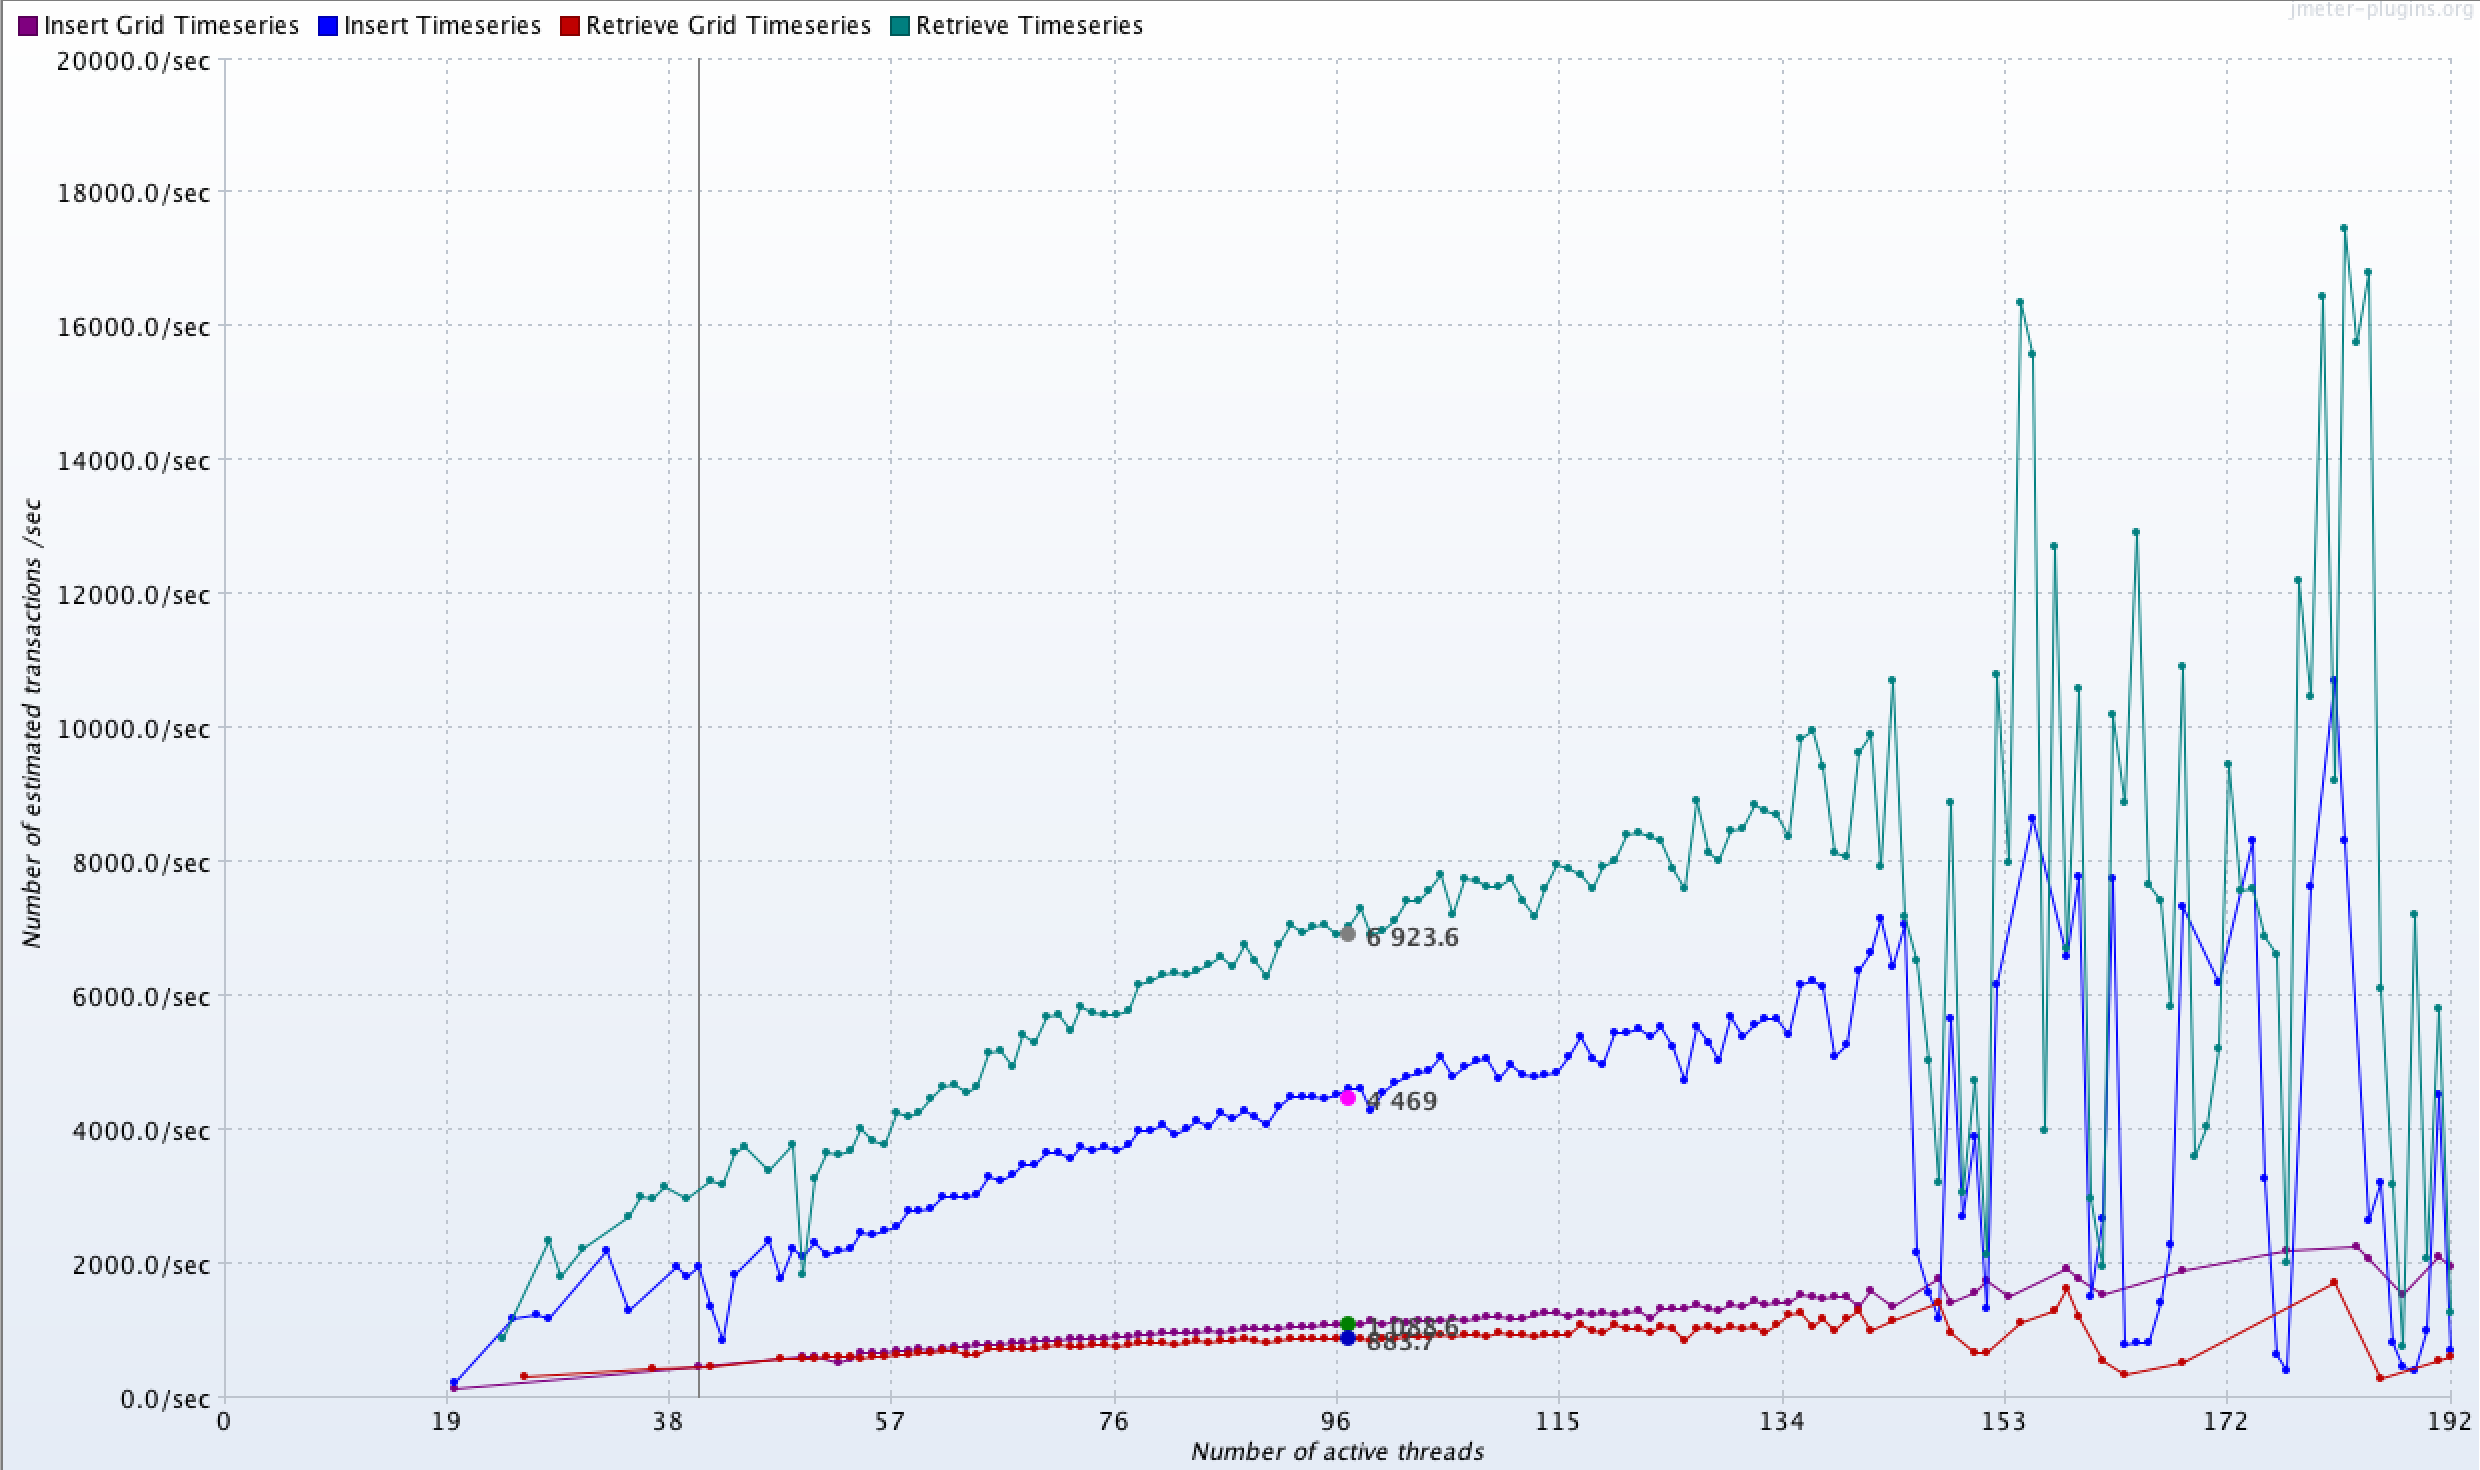
\includegraphics[width=1.0\textwidth]{results/obs/all/obs_all_15m_transaction_throughtput_vs_threads.png}
    \caption{Transaction throughput vs thread while load testing with 15-minute of data.}
    \label{fi:test_obs_all_15m_throughtput}
\end{figure}

\cref{fi:test_obs_all_15m_throughtput} shows the total server's transaction throughput against the number of active threads.
The formula for total server transaction throughput is \emph{active threads per second / one thread response time} \cite{ApacheSoftwareFoundationJMeter:Plugin}.
It shows the statistical maximum possible number of transactions based on the number of active threads accessing the application at a given time. This estimates the transaction throughput based on the latency of requests against the number of active threads at a given time. We can assume that the highest number of active threads occur at the peak time of the load testing. However, the number of latency samples are limit with the higher number of active threads. Consequently, in \cref{fi:test_obs_all_15m_throughtput} we can see missing data points, and spikes with graph drawing with available data points. Further we can analyze this graph against \cref{fi:test_obs_all_15m_response_vs_threads}, and derive this output based on latency fluctuation in that graph. By combining the \cref{fi:test_obs_all_15m_latency}, this graph shows that the throughput of the system gets increased without much change in the latency, thus it proves the scalability of the \acrshort{wdias}.


%%%%%%%%%%%%%%%%%%%%%%%%%%%%%%%%%%%%%%%%%%%%%%%%%%%%%%%%%%%%%%%%%%%%%%%%%%%%%%%%
\subsection{Load Testing with 15-minute Resolution Data with Auto Pod Scaling}
\label{subse:obs_test_plan_all_auto_15min}

Here we did the performance test plan with 15-minute resolution data, which is similar to the above section. However, during the test plan, we enabled the K8s auto-scaling only for higher resource utilized microservices, as explained in \cref{subse:test_plan_metrics}. While performing the above test plans, we noticed the import-ascii-grid-upload microservice is using lots of CPU, and the adapter-grid microservice is using lots of memory. Before starting the test plan, we configured auto-scaling for the import-ascii-grid-upload microservices. However, the adapter-grid microservice is a consistent service for storing netCDF files. If we want to enable the auto-scaling for the service, all microservice instances of adapter-grid need to share data via shared storage. Since \acrshort{eks} does not support multiple reads and writes support volumes \cite{LinuxFoundationKubernetesVolumes}, we are unable to enable auto-scaling during the test plan. But some of other \acrshort{k8s} platforms support multiple reads, and writes volumes. However, the test plan performed approximately \num{311e3} of almost similar sample requests during the above sections.

\begin{table}[ht]
\caption{Throughput and latency of load test with 15-minute data while enabled \acrshort{k8s} auto-scaling}
\footnotesize
\begin{tabulary}{\linewidth}{|L|R|R|R|R|R|R|R|R|}
\hline
\textbf{Label} & \textbf{Samples} & \textbf{Avg} & \textbf{Min} & \textbf{Max} & \textbf{90\% Line} & \textbf{Std.Dev.} & \textbf{Error} & \textbf{RPS} \\ \hline
Insert Timeseries & 71727 & 34 & 13 & 1777 & 27 & 118.78 & 0.00\% & 40.5 \\ \hline
Retrieve Timeseries & 71693 & 7 & 5 & 1608 & 9 & 18.72 & 0.00\% & 40.5 \\ \hline
Insert Grid & 7968 & 87 & 77 & 233 & 98 & 14.07 & 0.18\% & 4.5 \\ \hline
Retrieve Grid & 7965 & 89 & 63 & 1694 & 110 & 37.79 & 0.00\% & 4.5 \\ \hline
Query: Location & 71704 & 1 & 0 & 203 & 2 & 2.05 & 0.00\% & 40.5 \\ \hline
\textbf{TOTAL} & 310734 & 130 & 0 & 1777 & 501 & 212.35 & 0.00\% & 175.3 \\ \hline
\end{tabulary}
\label{tab:obs_all_auto_15_min_summary}
\end{table}

\cref{tab:obs_all_auto_15_min_summary} shows the response latency summary details and \acrshort{rps} as explained in \cref{subse:obs_test_plan_all_15min}. If we analyzed the performance of the auto-scaling enabled microservice, the average grid data insertion latency was reduced from 91 milliseconds to 87 milliseconds. Also, we can notice that the error percentage reduced from 1.42\% to 0.18\%. Since the standard deviation also reduced, we can conclude that the latencies are closer to the average latency. Further, these improvements in insert grid timeseries data seem to affect the output of retrieve grid timeseries data as well, and decrease the latency from 118 milliseconds to 89 milliseconds. When it comes to scalar and vector timeseries data insertion, latency was increased a bit. However, we can notice that, the retrieval of scalar and vector timeseries latency improved from 23 milliseconds to 7 milliseconds. Specially, the latency for query location timeseries metadata was improved from 3 milliseconds to 2 milliseconds. It was constant with 3 milliseconds in previous load testings. Other than inserting scalar and vector data, other test cases standard deviation was improved, and we can conclude that the overall system performance is enhanced when auto-scaling is enabled.

\begin{figure}[htp]
    \centering
    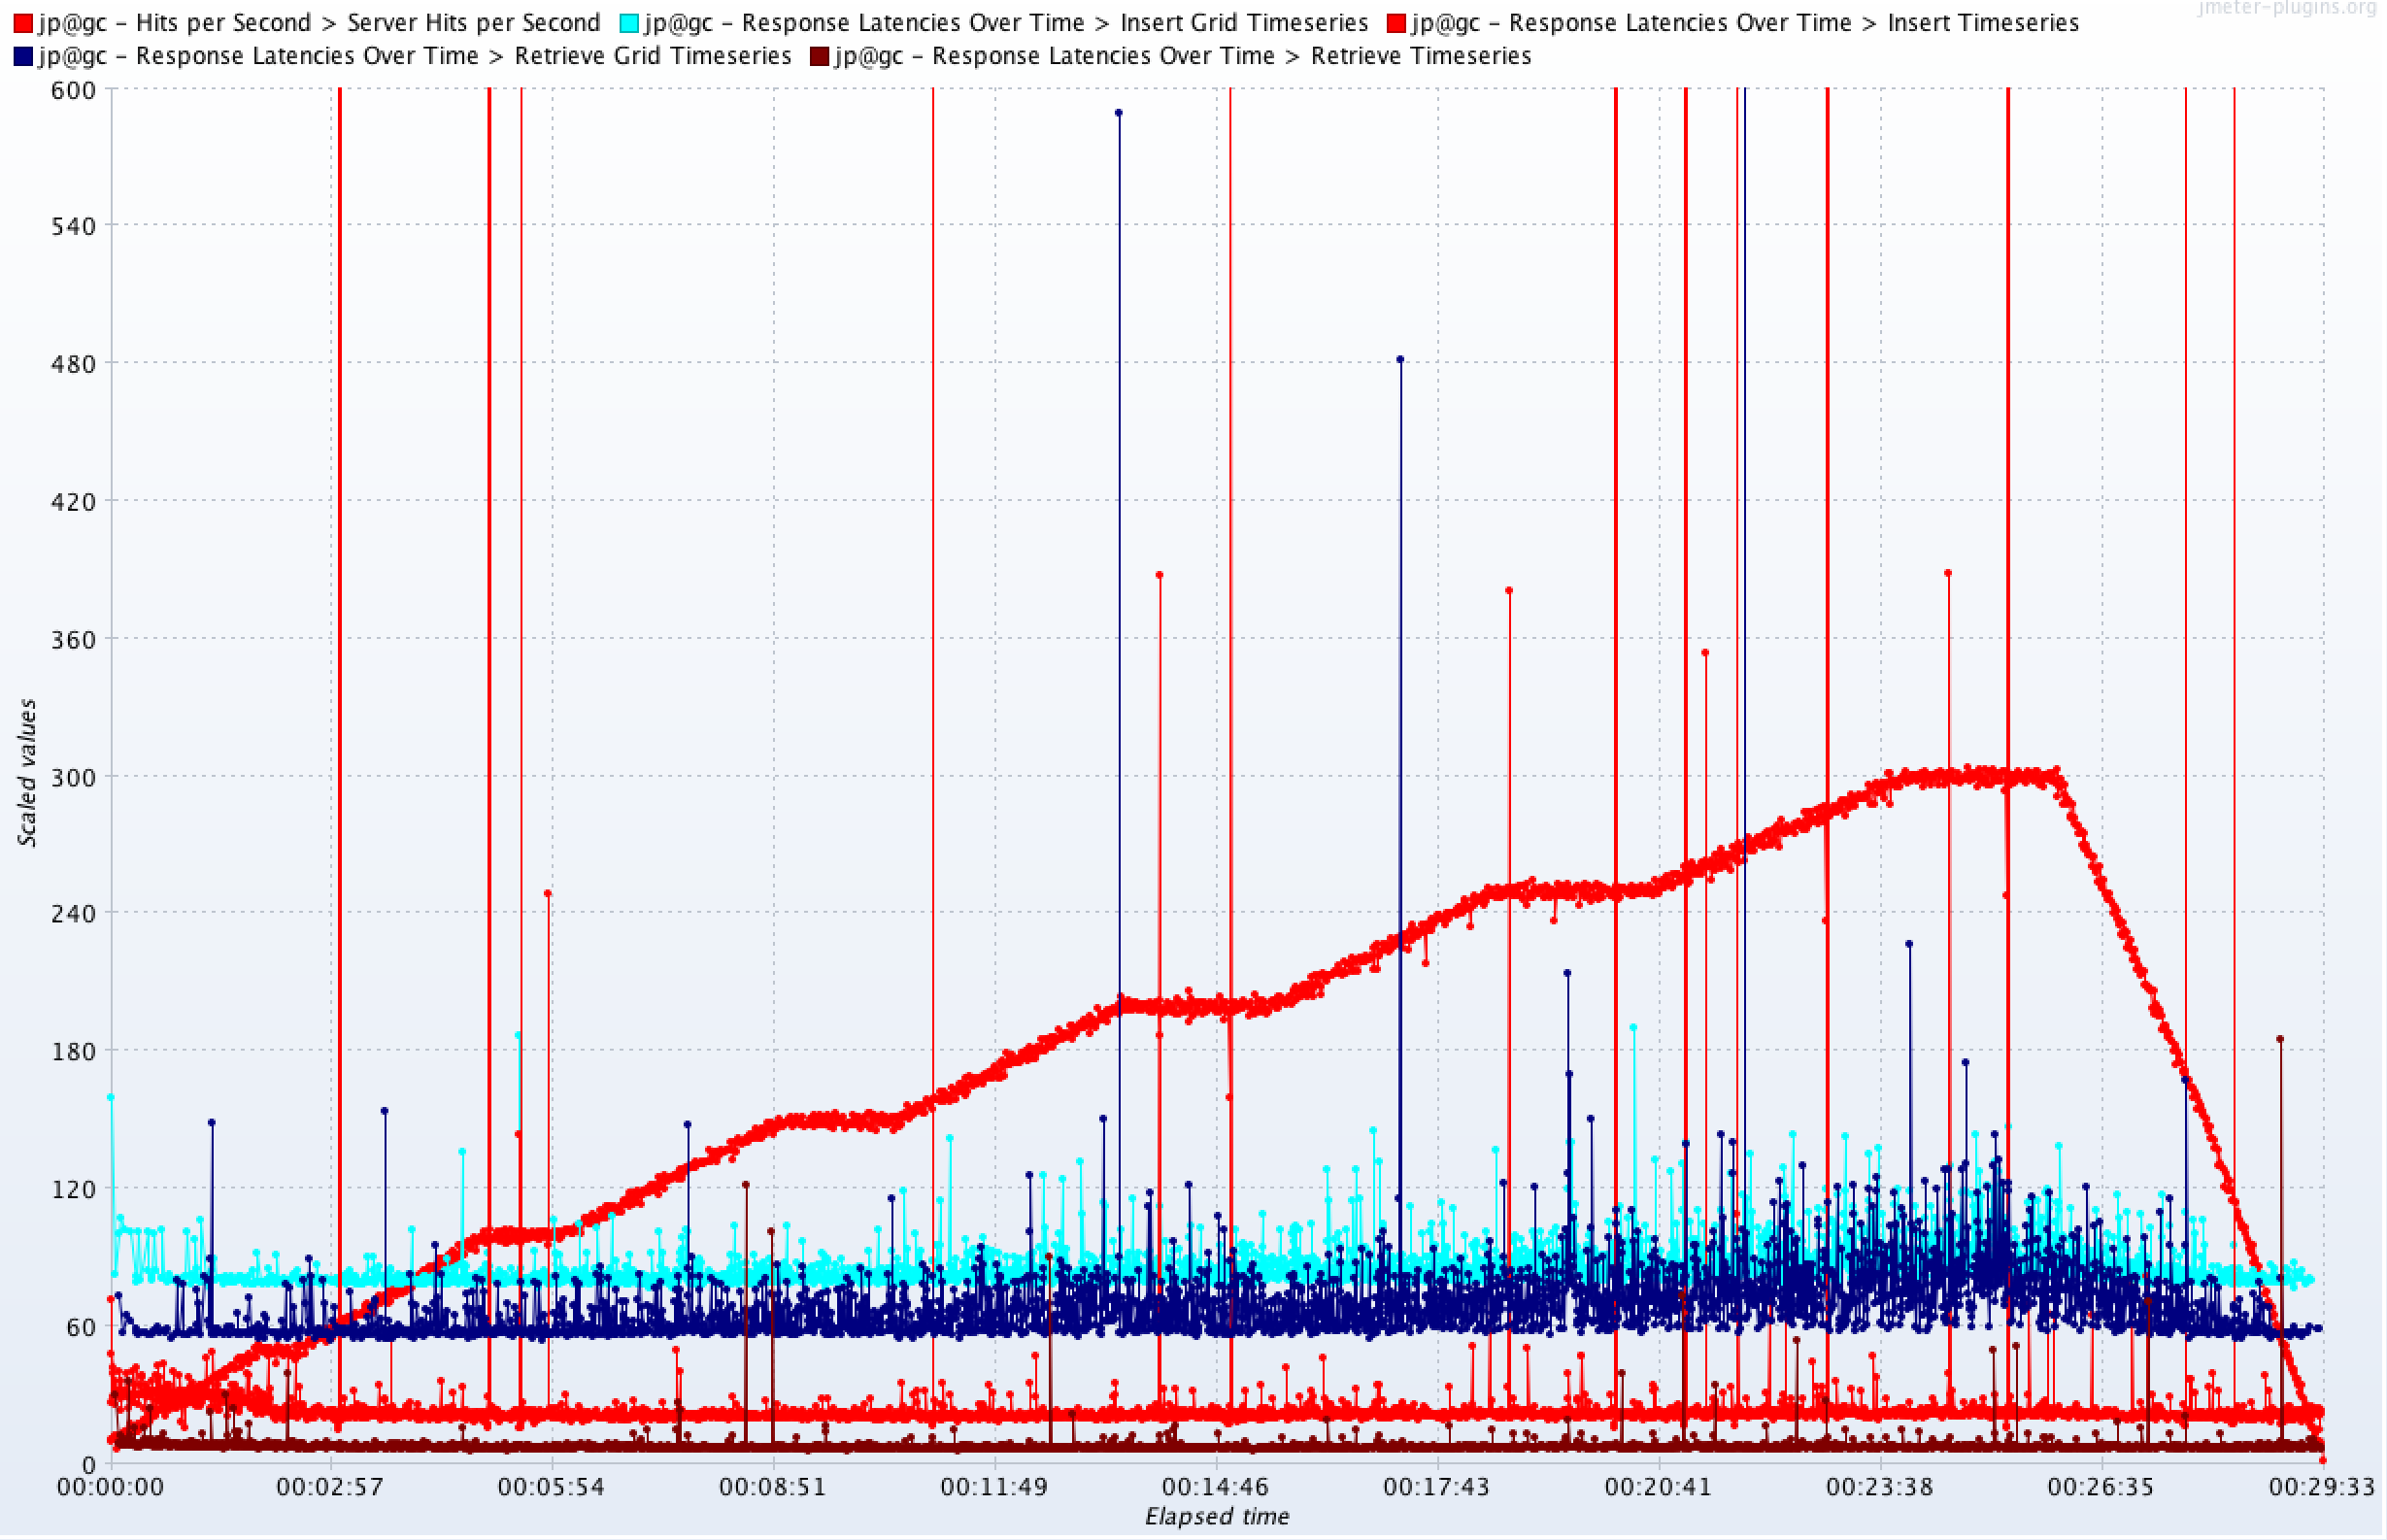
\includegraphics[width=1.0\textwidth]{results/obs/all_auto/obs_all_auto_15m_res_latencies_against_hits.png}
    \caption{Latency against server hits while load testing with 15-minute of data with enabled auto-scaling.}
    \label{fi:test_obs_all_auto_15m_latency}
\end{figure}
\cref{fi:test_obs_all_auto_15m_latency} graph provides an overview of the variation of latency over the elapsed time of the test plan against the number of server hits per second for 15-minute data while auto-scaling enabled for \acrshort{k8s}. According to the graph, the \acrshort{wdias} was able to keep the latency constant all over the elapsed time.
When compared to \cref{fi:test_obs_all_15m_latency} without auto-scaling, we can see lesser latency spikes throughout the test period.

\begin{figure}[htp]
    \centering
    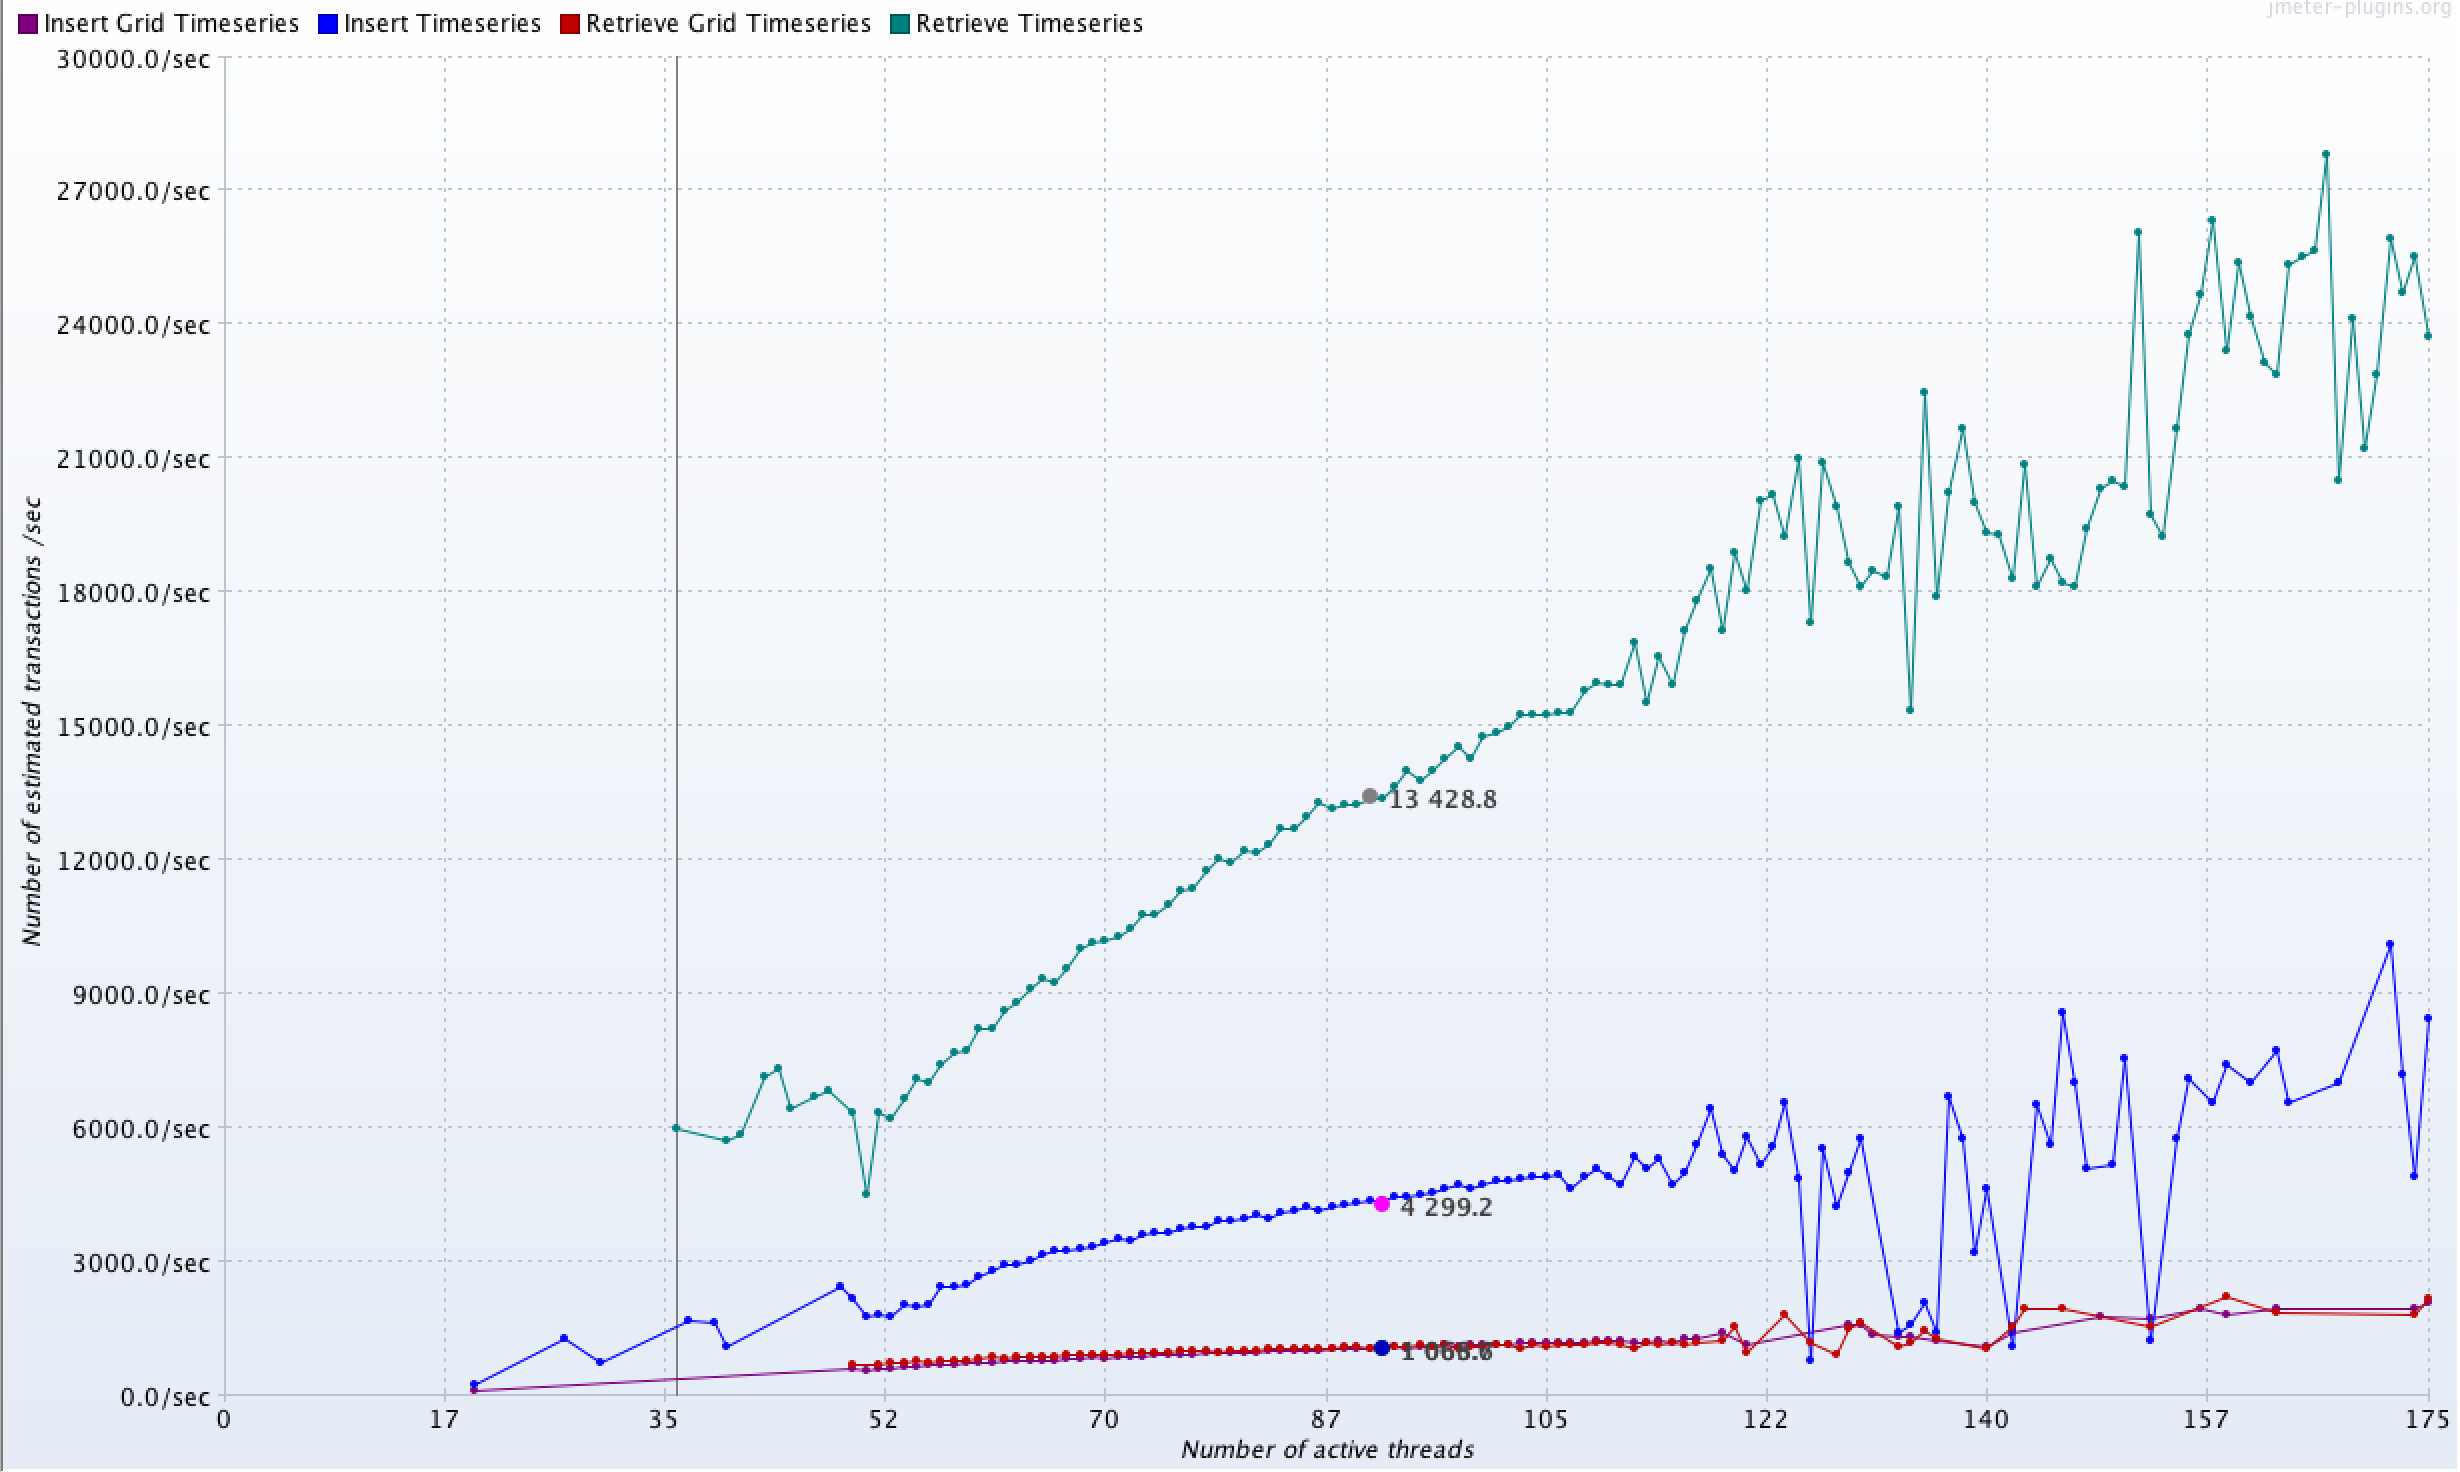
\includegraphics[width=1.0\textwidth]{results/obs/all_auto/obs_all_auto_15m_transaction_throughtput_vs_threads.png}
    \caption{Transaction throughput vs threads while load testing with 15-minute of data with enabled auto-scaling.}
    \label{fi:test_obs_all_auto_15m_throughtput}
\end{figure}

\cref{fi:test_obs_all_auto_15m_throughtput} shows the total server's transaction throughput against the number of active threads. When compared to \cref{fi:test_obs_all_15m_throughtput} without auto-scaling, the estimated throughput with a higher number of active threads becomes stable, according to the graph. Thus, we can conclude that enabling auto-scaling also improves the throughput by supporting a higher number of active threads. We can see fluctuation when increase the number of active threads due to lack of sample latency with higher number of active threads during the peak of load testing. Further, we can see estimated throughput for insert and retrieve grid data also increased by a small factor, and it more smooth than 15-minute data load testing without auto-scaling. During the next paragraphs, we will discuss the resource usage while running the test plan while enabling the auto-scaling.

\begin{figure}[htp]
    \centering
    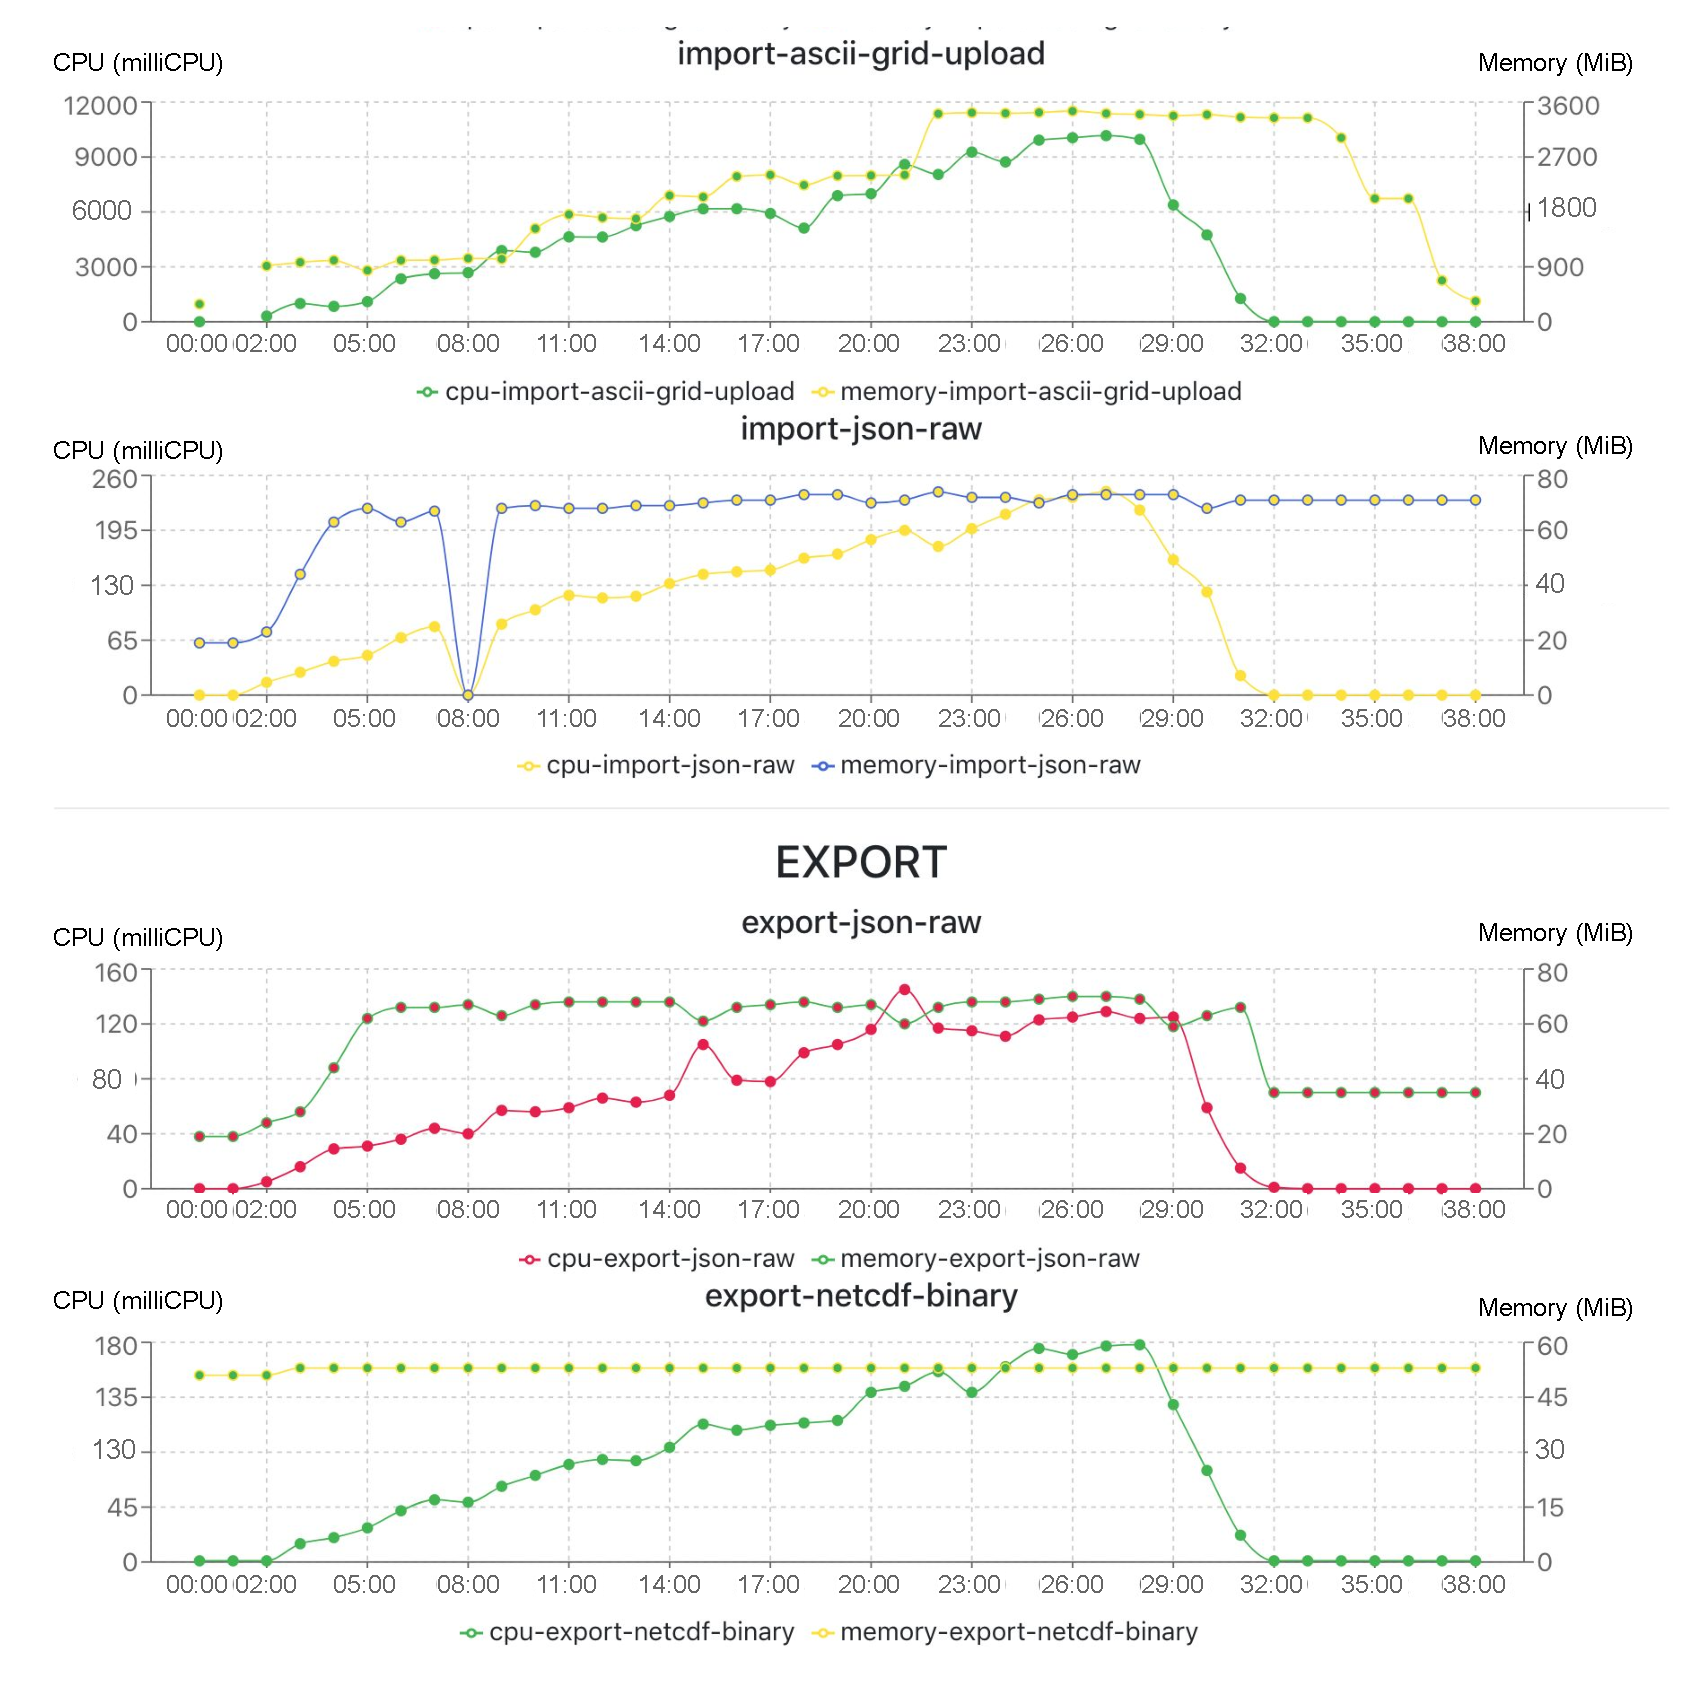
\includegraphics[width=1.0\textwidth]{results/obs/all_auto/obs_all_auto_15m_import_export_res.pdf}
    \caption{Load testing with auto-scaling resource usage of import and export modules over time.}
    \label{fi:obs_all_auto_15m_import_export_res}
\end{figure}

\cref{fi:obs_all_auto_15m_import_export_res} shows the CPU usage and memory usage for import timeseries modules and export timeseries modules with 1-minute resolution. We show the CPU usage with milli CPUs \cite{LinuxFoundationKubernetes:Containers} (1 CPU = 1000m CPUs) and the memory usage shown with Megabytes (Mi) \cite{LinuxFoundationKubernetes:Containers} in the graphs. Noticeably, the import-ascii-grid-upload microservice used around 10 CPUs at the peak time while using 3.6 Gigabytes (Gb) of memory. Another important fact is, after the test cases finished, the \acrshort{wdias} cooled down the system via K8s auto-scaling and released the resources. Thus, we can see the elasticity of the \acrshort{wdias} according to the workload.

\begin{figure}[htp]
    \centering
    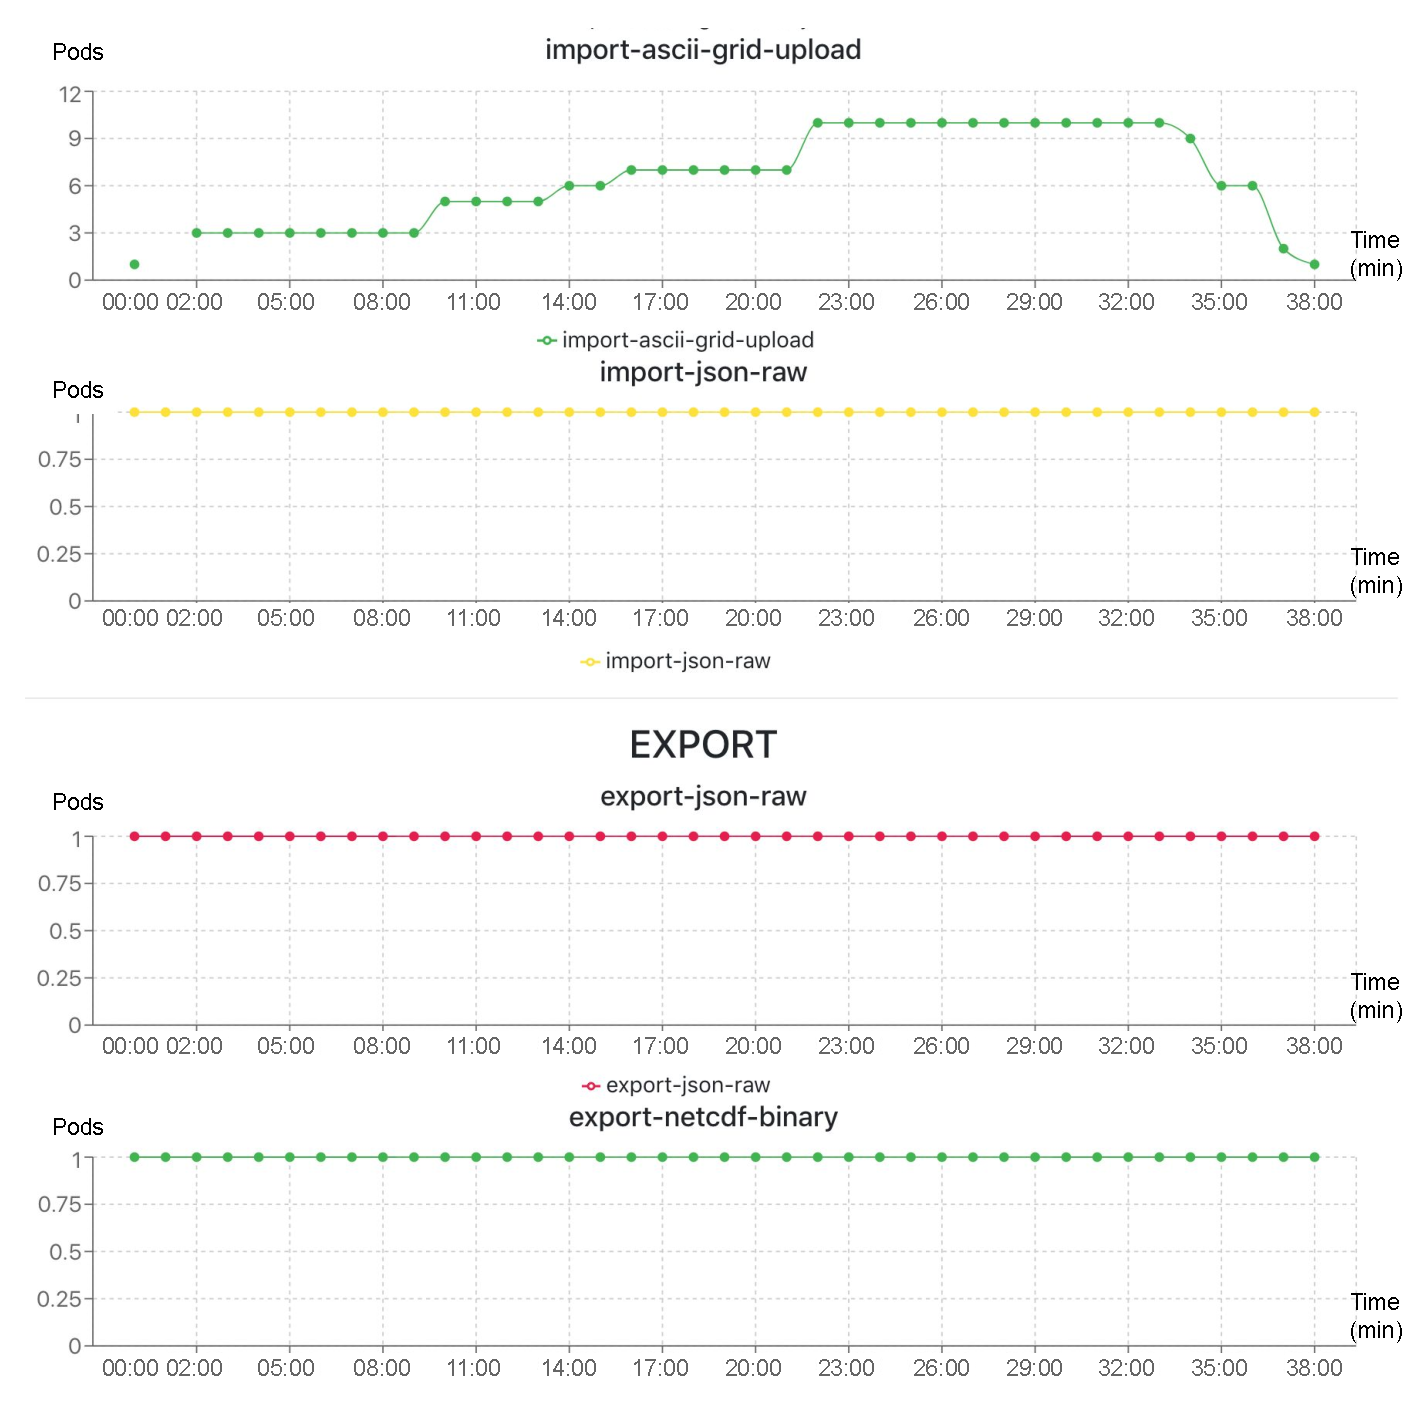
\includegraphics[width=1.0\textwidth]{results/obs/all_auto/obs_all_auto_15m_import_export_pods.pdf}
    \caption{Load testing with auto-scaling number of pods of import and export modules over time.}
    \label{fi:obs_all_auto_15m_import_export_pods}
\end{figure}

\cref{fi:obs_all_auto_15m_import_export_pods} shows the number of import-ascii-grid-upload pods scheduled overtime during the test plan. As mentioned in the previous paragraph, we enabled the auto-scaling with a maximum of 10 pods and 80\% recommended CPU usage. As the graph shows, we scheduled three pods before initialing the test plan. When the workload increased, K8s spawned new pods while keeping the total CPU utilization up to 80\%, as we configured above. After K8s spawned ten maximum pods, it stopped spawning new pods. However, each pod was able to vertical scale up to the limit of 2 CPUs. Even we saw the resources released after the peak load, but the number of pods did not decrease according to the graph. K8s has a threshold of reducing the number of pods, and it waits for 5 minutes before terminating a pod after a resource is released.

\begin{figure}[htp]
    \centering
    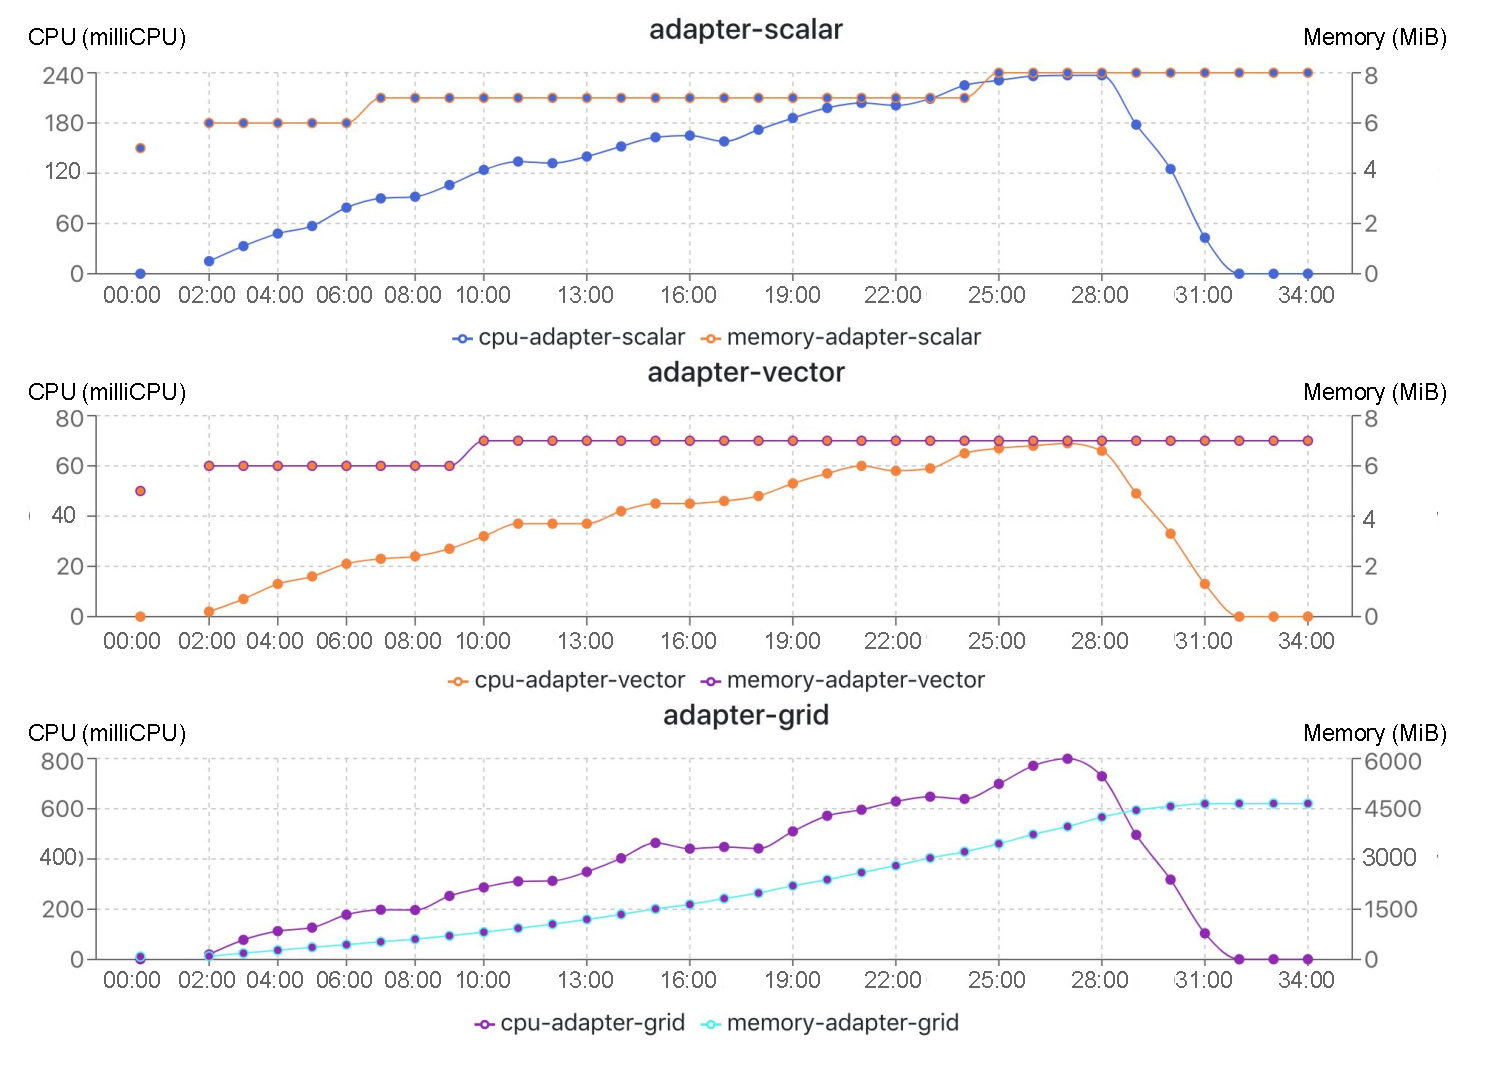
\includegraphics[width=1.0\textwidth]{results/obs/all_auto/obs_all_auto_15m_adapter_dbs_res.pdf}
    \caption{Load testing with auto-scaling resource usage of database adapters over time.}
    \label{fi:obs_all_auto_15m_adapter_dbs_res}
\end{figure}

\cref{fi:obs_all_auto_15m_adapter_dbs_res} shows the resource utilization of database adapters in the \acrshort{wdias}. The scalar adapter and vector adapter are not getting heavy load since they only process a scalar array of data points. However, we can see the CPU usage over time increased according to the test plan workload and cool down after the peak. For the grid adapter, the CPU resource utilization increased and cooled down similarly to other adapters. However, the memory resources are not released due to the caching of netCDF files by the application.

%%%%%%%%%%%%%%%%%%%%%%%%%%%%%%%%%%%%%%%%%%%%%%%%%%%%%%%%%%%%%%%%%%%%%%%%%%%%%%%%
\subsection{Query Module Load Test}
\label{subse:obs_test_plan_query_15min}

This \cref{subse:obs_test_plan_query_15min} discussed the query test plan performance. During the test plan, we performed multiple information retrievals queries such as queries over locations, parameters, and timeseries, which we described in the test planning phase. The test plan performed approximately \num{123e3} of sample requests only with the query microservice during the test period. We performed the query test plan over 5 minutes with a higher number of requests than other test plans with a peak of 600 hits per second.

\begin{table}[ht]
\caption{Throughput and latency of query test cases with 15-minute data}
\footnotesize
\begin{tabulary}{\linewidth}{|L|R|R|R|R|R|R|R|R|}
\hline
\textbf{Label} & \textbf{Samples} & \textbf{Avg} & \textbf{Min} & \textbf{Max} & \textbf{90\% Line} & \textbf{Std.Dev.} & \textbf{Error} & \textbf{RPS} \\ \hline
* → Locations & 11462 & 992 & 5 & 17569 & 1740 & 704.67 & 0.00\% & 38.3 \\ \hline
Area → Locations & 11390 & 599 & 2 & 16755 & 1047 & 514.68 & 0.00\% & 38.1 \\ \hline
Location → Parameters & 11350 & 666 & 1 & 16821 & 1179 & 632.86 & 0.00\% & 38.0 \\ \hline
Locations → Parameters & 11305 & 659 & 1 & 17459 & 1149 & 678.55 & 0.00\% & 37.8 \\ \hline
Location → Timeseries & 11269 & 647 & 2 & 32693 & 1102 & 746.51 & 0.00\% & 37.7 \\ \hline
Locations → Timeseries & 11237 & 669 & 1 & 32651 & 1162 & 889.18 & 0.00\% & 37.6 \\ \hline
Locations, Parameter → Timeseries & 11192 & 662 & 2 & 32806 & 1152 & 789.49 & 0.00\% & 37.4 \\ \hline
Area → Timeseries & 11135 & 820 & 2 & 33235 & 1461 & 877.68 & 0.00\% & 37.3 \\ \hline
Area, Parameter → Timeseries & 11084 & 864 & 1 & 16699 & 1584 & 751.00 & 0.00\% & 37.1 \\ \hline
*, Parameter → Timeseries & 11011 & 696 & 2 & 16689 & 1216 & 693.33 & 0.00\% & 36.8 \\ \hline
* → Timeseries & 10968 & 1473 & 24 & 18283 & 2467 & 912.45 & 0.00\% & 36.7 \\ \hline
\textbf{TOTAL} & 123403 & 794 & 1 & 33235 & 1536 & 789.76 & 0.00\% & 412.6 \\ \hline
\end{tabulary}
\label{tab:obs_query_15_min_summary}
\end{table}

\cref{tab:obs_query_15_min_summary} shows the response latency summary details. The average latency is much higher than the minimum value. Also, the summary reported higher maximum values as well. Standard deviation showed a quiet higher value, which means the response latency values are not closer to the average value. Noticeably, we cannot see any errors in the table, which means all the requests successfully process. The throughput is similar among all the requests. The performance of the query adapter depends on the performance of the document storage database performance and geo-indexing performance.

\begin{figure}[htp]
    \centering
    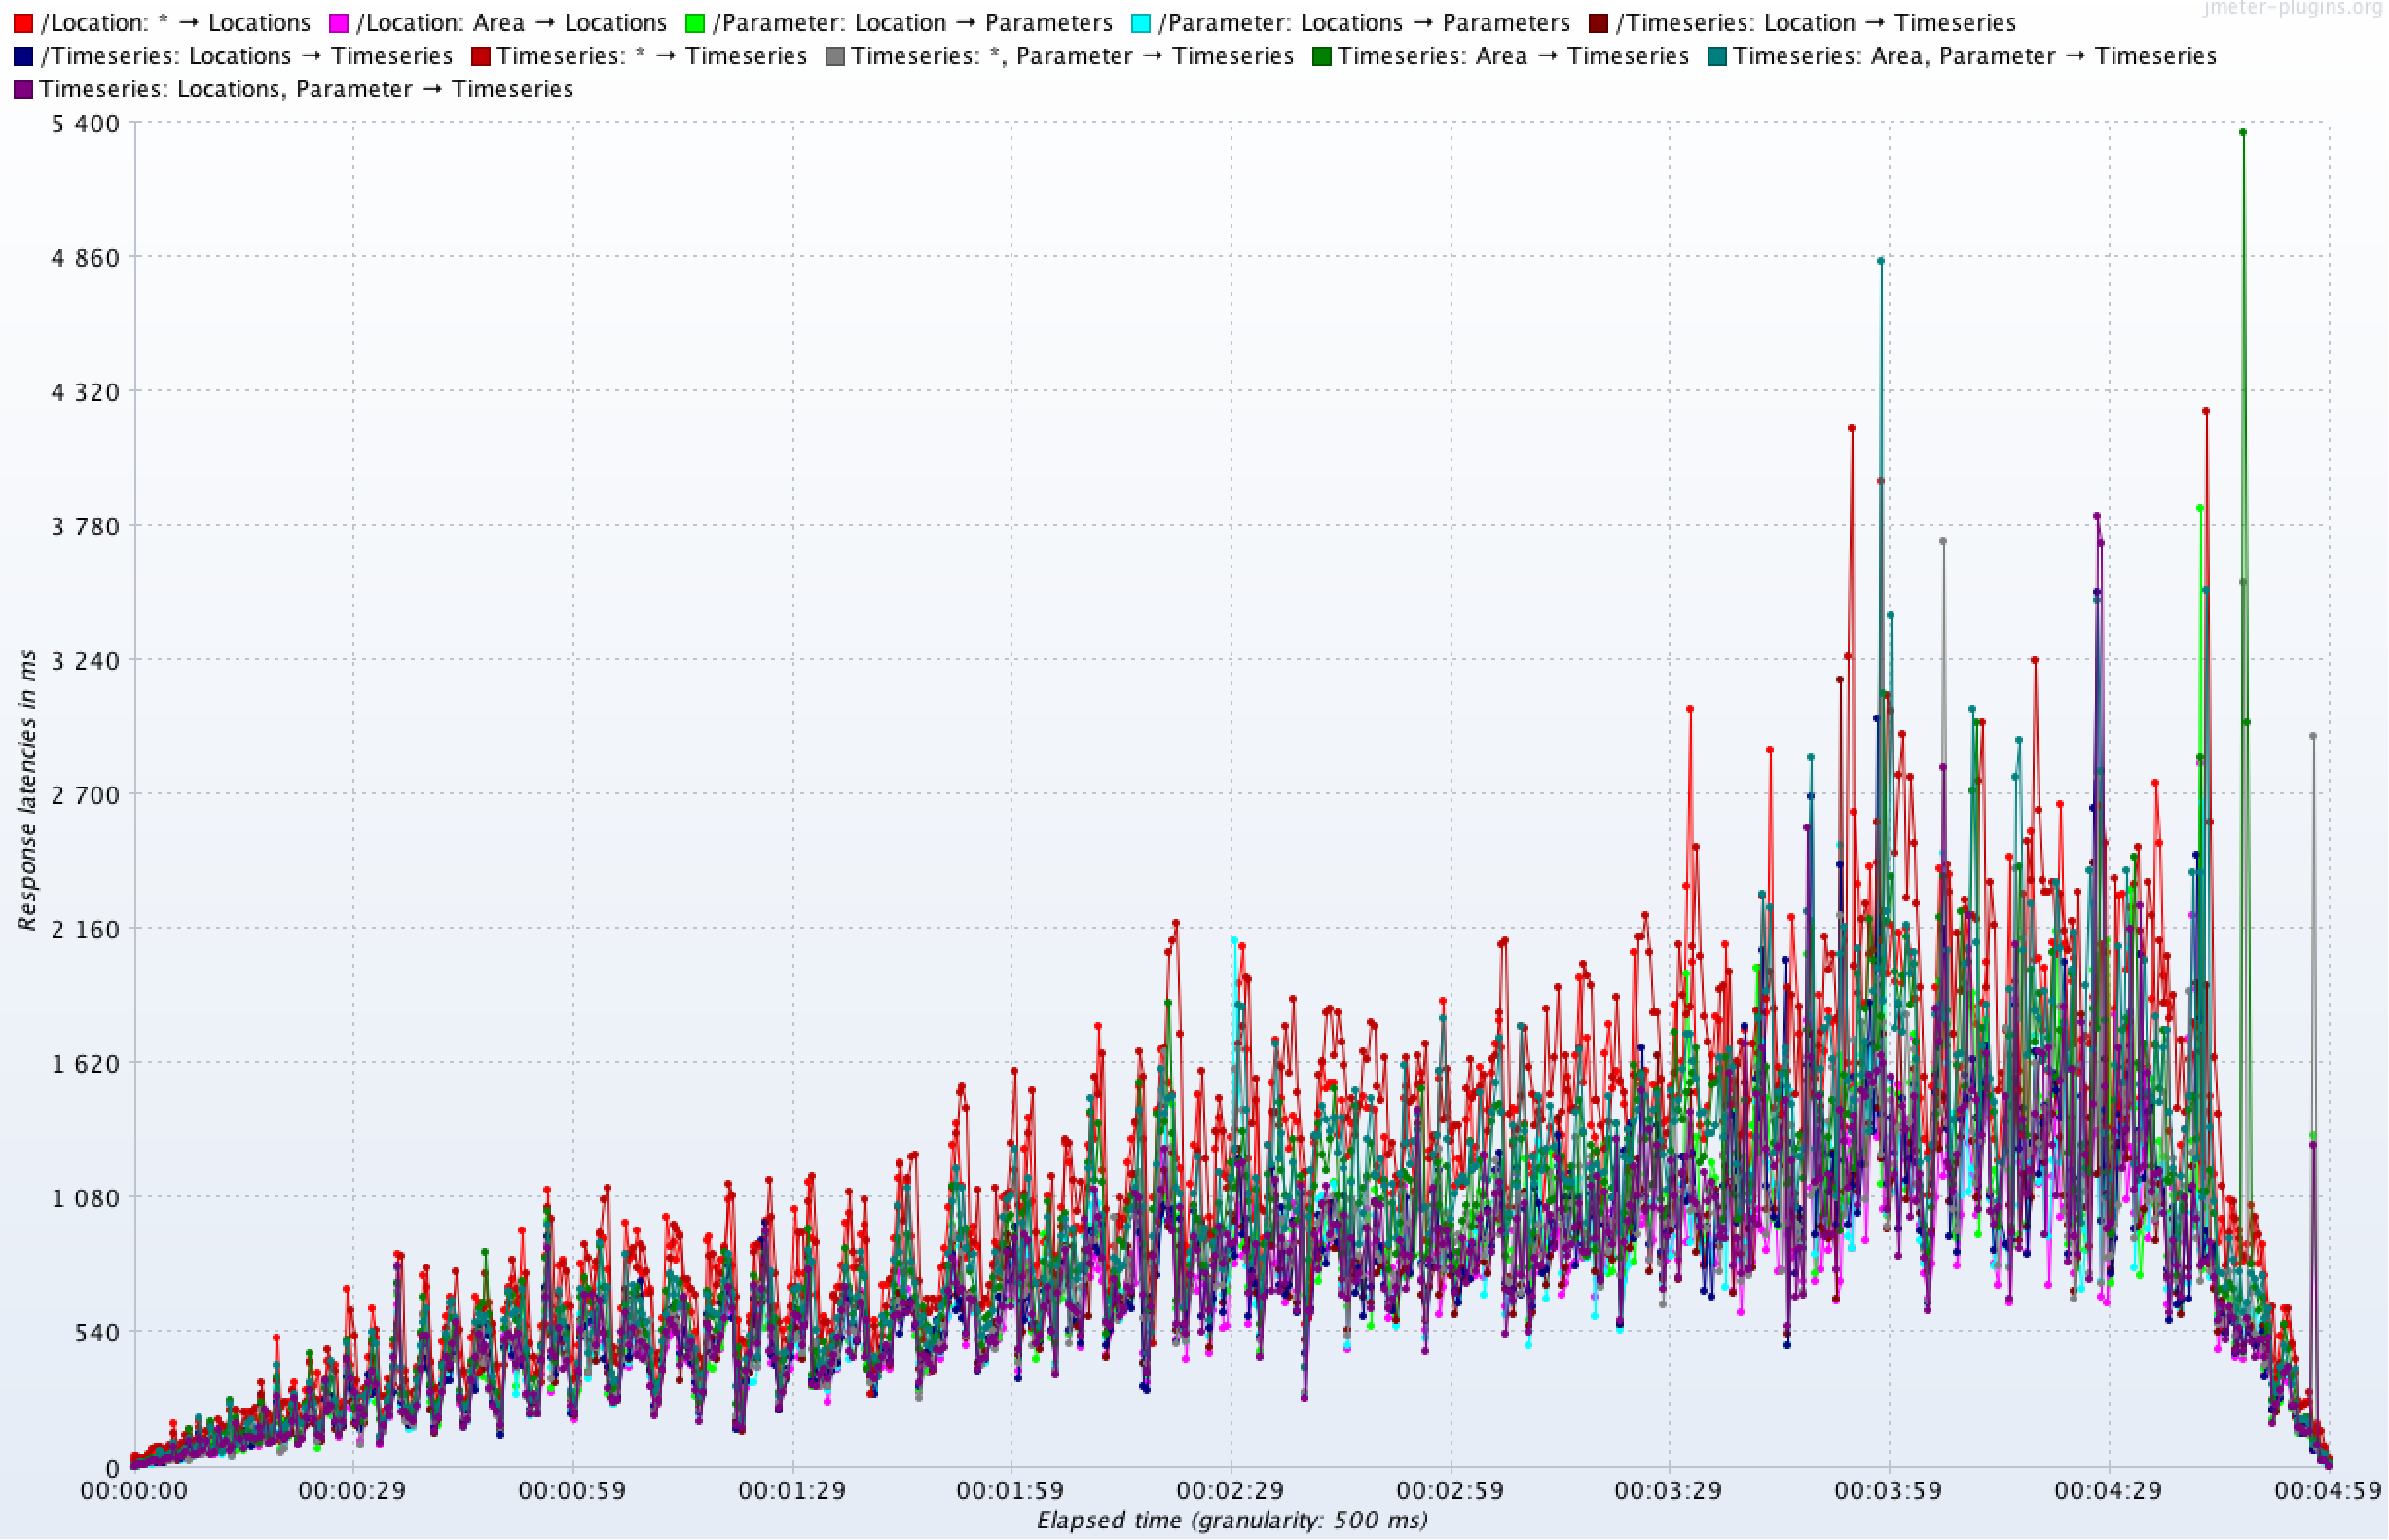
\includegraphics[width=1.0\textwidth]{results/obs/query/obs_query_5m_latency_over_time.png}
    \caption{Response latency over time while load testing query test over 5 minutes.}
    \label{fi:test_obs_query_5m_response_latency}
\end{figure}
\cref{fi:test_obs_query_5m_response_latency} shows the response latency overtime for the query test plan. When the number of requests gets higher, the latency also gets increased. Further, \cref{fi:test_obs_query_5m_response_times_vs_threads} shows the response latency against the number of active threads for the query test plan. When the number of server hits gets higher, the latency also increases. According to the figures, we can conclude that the performance of the query adapter depends on the database. Even if we increase the number of query adapter pods, the throughput of the microservice is not going to increase until we increase the performance by using the z-axis scaling of scale cube concept.

\begin{figure}[htp]
    \centering
    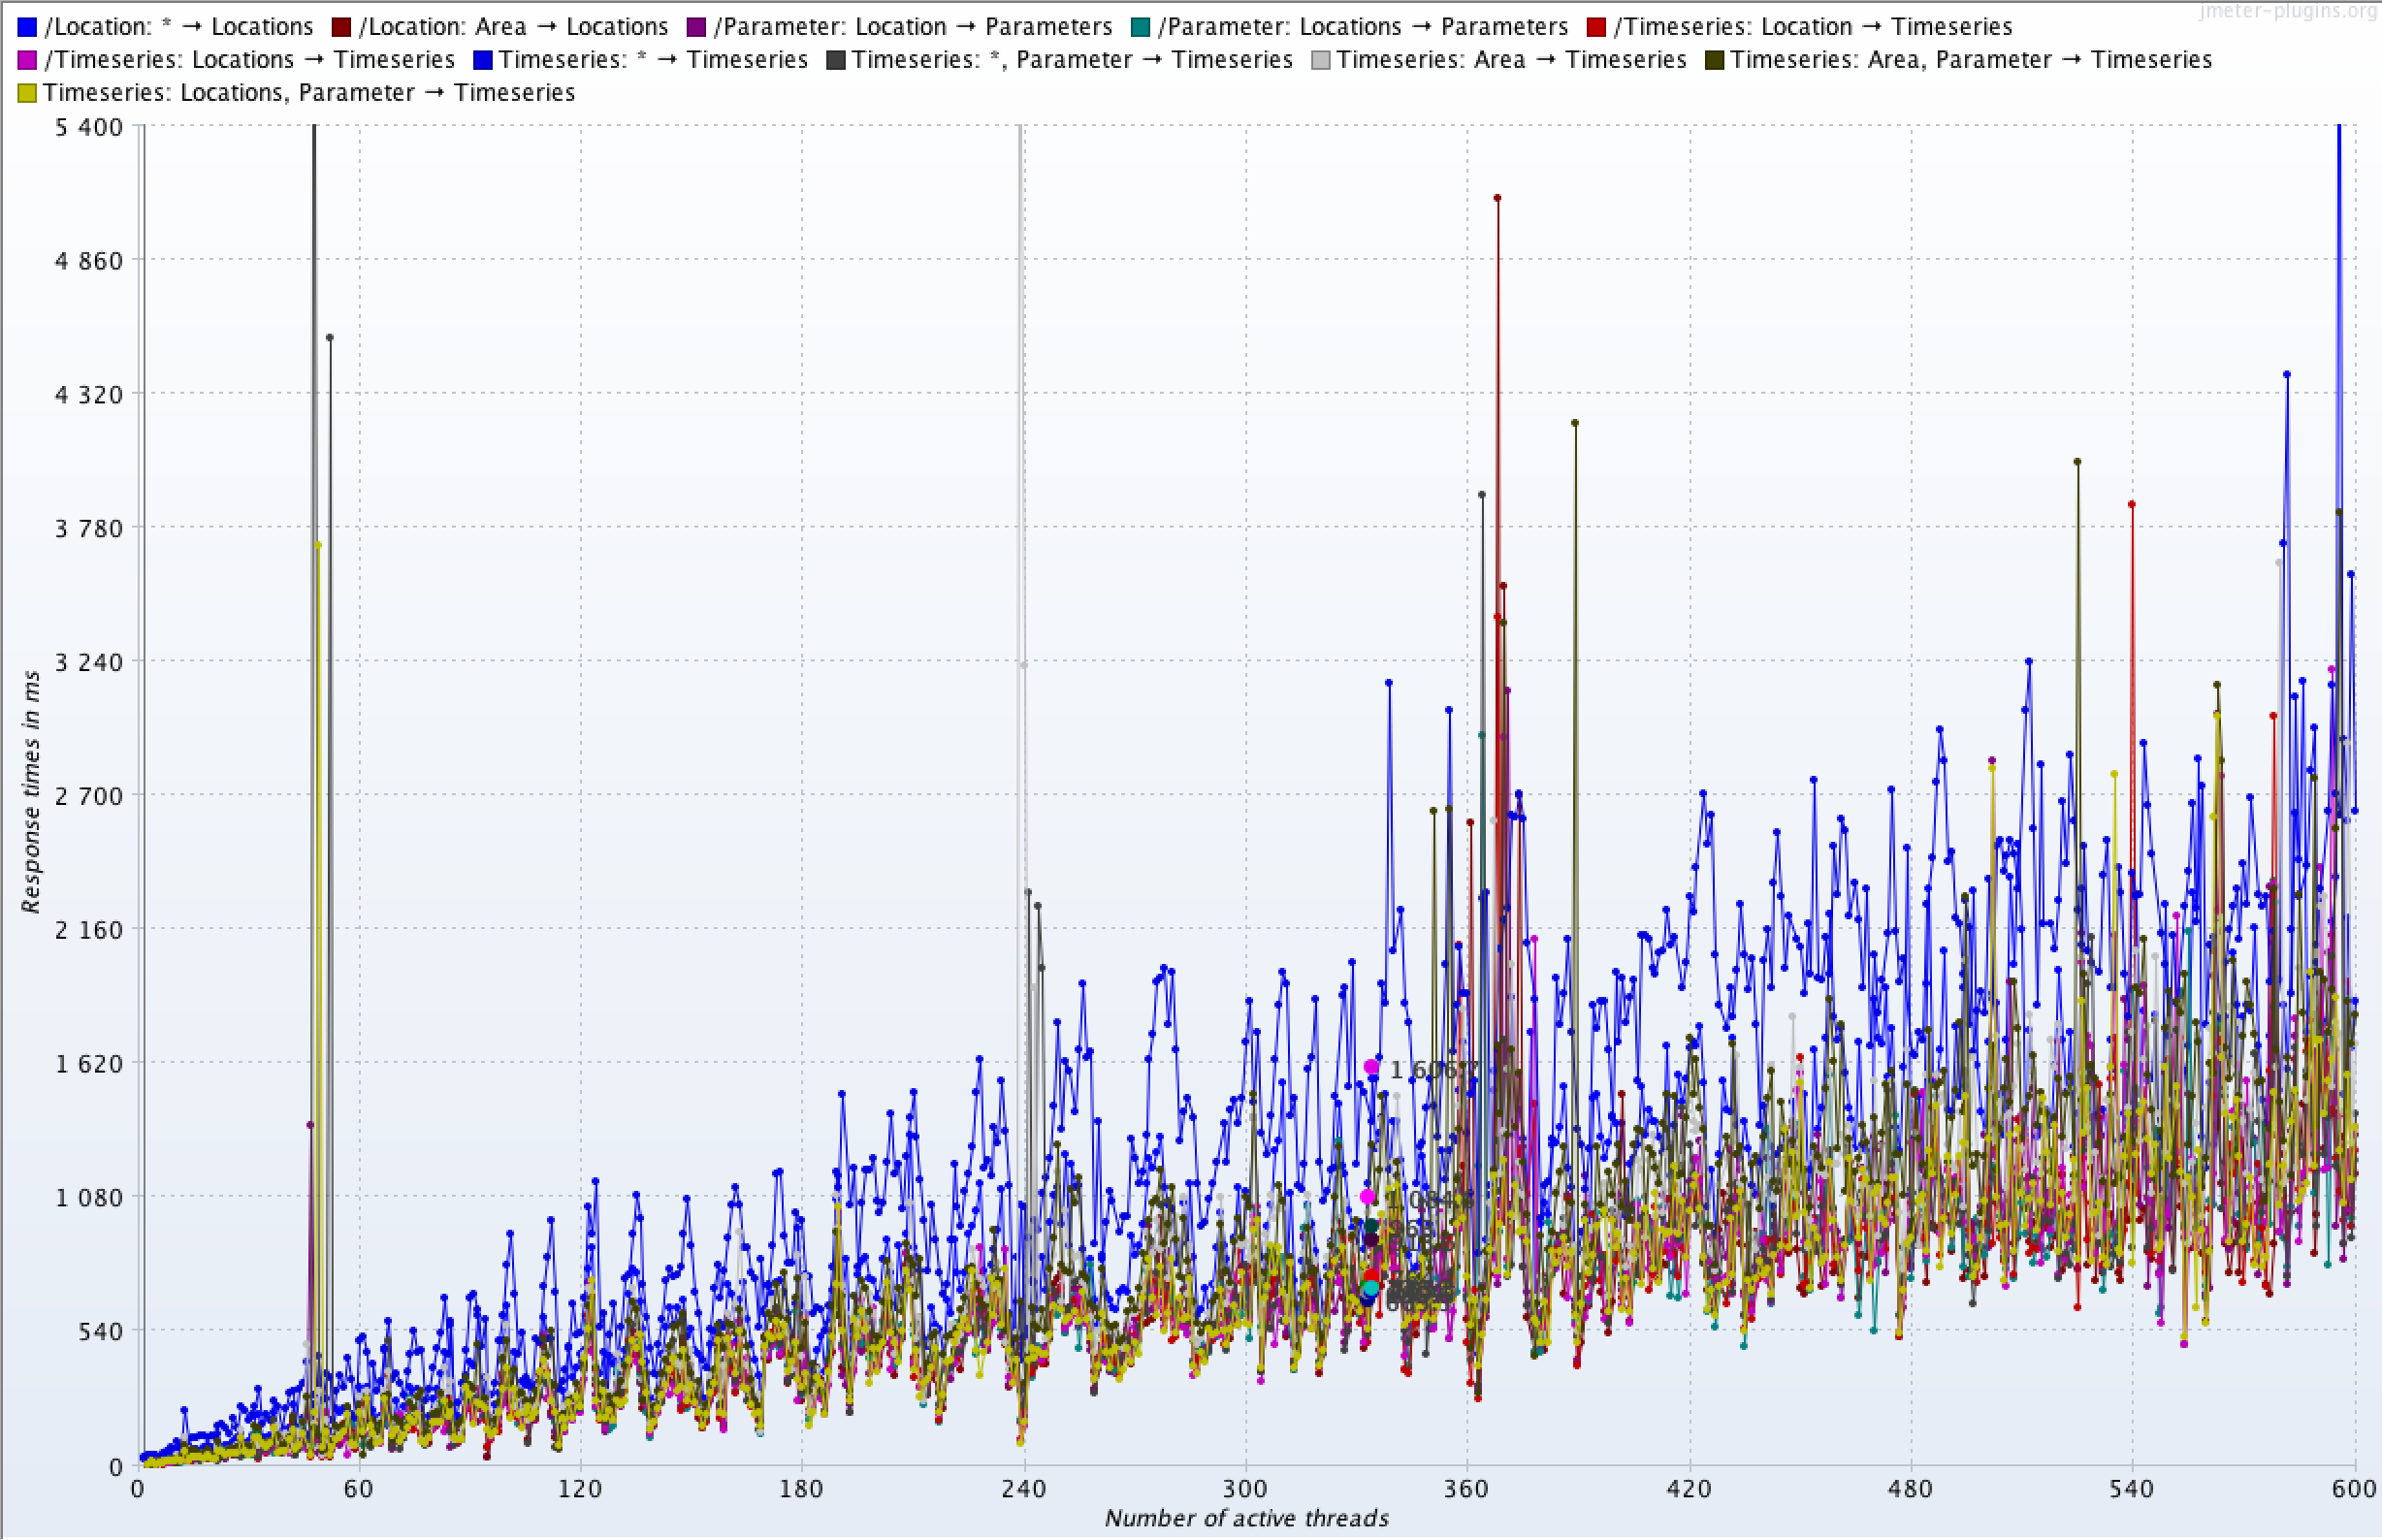
\includegraphics[width=1.0\textwidth]{results/obs/query/obs_query_5m_response_times_vs_threads.png}
    \caption{Response latency times vs threads load testing query test over 5 minutes.}
    \label{fi:test_obs_query_5m_response_times_vs_threads}
\end{figure}

Whenever the timeseries data is not found in the query adapter, it reads data from metadata adapter and index for search over timeseries metadata. We used the above mechanism to increase the performance with geo timeseries searches. The performance of the document storage can further improve with using its features like replication for high availability, and sharding for higher throughput.
We did not attempt those performance improvements during the test plan since it was beyond the scope of the research. However, the users of the \acrshort{wdias} system can enable such features and get higher performance.
